\documentclass[12pt,paper]{article}
\usepackage[utf8]{inputenc}
\usepackage[spanish]{babel}%lenguaje
\usepackage{amsmath}%operadores matemáticos
\usepackage{natbib}
\usepackage{gensymb}
\usepackage{graphicx}
\usepackage{subfigure}
\usepackage[hidelinks]{hyperref}
\usepackage{float}
\usepackage{physics}
\usepackage{longtable}
\usepackage{multirow}
\usepackage{hyperref}
\usepackage{subfig}
\usepackage[T1]{fontenc}
\usepackage{imakeidx}
\usepackage{xcolor}
\makeindex[columns=3, title=Alphabetical Index, intoc]
\usepackage[a4paper]{geometry}
\geometry{top=2.5cm, bottom=2.5cm, left=2.25cm, right=2.75cm}

\begin{document}

\begin{titlepage}
\centering
{
\includegraphics[width=0.3\textwidth]{logo-UGR-color-vertical.jpg}\par}
\vspace{1cm}
{\bfseries\LARGE Facultad de Ciencias \par}
\vspace{1cm}
{\scshape\Large Grado en Física - Física Computacional. \par}
\vspace{1cm}
{\scshape\textbf{\Large Voluntario 3:  Simulación de la ecuación de Schrödinger dependiente del tiempo para el oscilador armónico cuántico.} \par}
\vspace{1cm}
{\itshape\Large  \par}

{\small Autores: \par}
{\Large Alonso José Suárez Reza \par}\vspace{0,2cm}
\small Física Computacional. \\ 
\small 16 de Julio de 2024.
\vspace{1 cm} 
\newpage
\tableofcontents
\clearpage
\end{titlepage}

\newpage
\section{Fundamento teórico.}
En física cuántica o mecánica cuántica, la ecuación de Schrödinger es de gran relevancia ya que nos permite entender cómo evoluciona el estado físico, representado por una función de onda, de partículas cuánticas. Sobretodo computacionalmente podemos visualizar y simularlo para comprender el modelo.\\

La forma general de la ecuación de Schrödinger dependiente del tiempo es:
\begin{equation*}
    i \hbar \frac{\delta}{\delta t} \phi(\Vec{r},t) = \hat{H} \phi(\Vec{r},t)
    \label{eq1}
\end{equation*}
donde i es la unidad imaginaria, $\hbar$ la constante de Planck dividida por 2$\pi$, $\phi(\Vec{r},t)$ la función de onda que describe el estado físico de la partícula, y $\hat{H}$ el operador lagrangiano.\\

Para una partícula no relativista unidimensional de función de onda compleja $\phi(x,t)$ con masa $m$ y $H$ el operador Hamiltaniano hermítico, podemos escribir la ecuación de Schrödinger cómo:
\begin{equation}
    i \hbar \frac{\delta}{\delta t} \phi(x,t) = H \phi(x,t) = [-\frac{\hbar^2}{2m} \frac{\delta^2}{\delta x^2} + V(x)] \phi(x,t)
\end{equation}\\

Siendo la solución general de $\phi(x,t) = e^{i(t-t_0)H} \phi(x,t_0)$.\\

Definimos los siguientes valores ya considerando el caso de una partícula unidemensional no relativista:
\begin{itemize}

    \item La densidad de probabilidad de una función $\phi(x,t)$:
    \begin{equation}
        P(x,t) = \abs{\phi(x,t)}^2
    \end{equation}
    
    \item La densidad de probabilidad de encontrar a la partícula el intervalo [a, b] y en el instante t:
    \begin{equation}
        P(a \leq x \leq b) = \int_a^b\abs{\phi(x,t)}^2dx
    \end{equation}
    \item La norma, para un sistema compuesto únicamente por una partícula, como es el nuestro, la probabilidad total de encontrar la partícula en algún punto del espacio, en cualquier instante t, debe ser igual la unidad y viene definido por P en el mismo espacio definido por $[a,b]$.
    
    \item El valor medio de una variable a o operador cualquiera A $<a>$ o $<A>$:
    \begin{equation*}
        <a> = \int_a^b\phi(x,t)^*a\phi(x,t)dx \hspace{2mm} ó \hspace{2mm} <A> = \int_a^b\phi(x,t)^*A\phi(x,t)dx
    \end{equation*}
    siendo $\phi(x,t)^*$ el conjugado de la función de onda $\phi(x,t)$.
    
    \item El operador momento del sistema $p$:
    \begin{equation}
        p = -i \hbar \frac{\delta}{\delta x}
    \end{equation}
    
    \item El hamiltoniano del sistema $H$:    
    \begin{equation}
        H = \frac{p^2}{2m} + V(x)
    \end{equation}
    
    
    
    \item El principio de Heisenberg:
    \begin{equation}
        \Delta x \Delta p \geq \frac{\hbar}{2}
    \end{equation}
    siendo $\Delta A$ para cualquier operador/variable de la forma:
    \begin{equation*}
        \Delta A = (<A^2>-<A>^2)
    \end{equation*}
    
\end{itemize}

Para realizar los cálculos numéricos y para evitar el uso continuado de tanto $m$ cómo $\hbar$ se va realizar el siguiente cambio de variable: $t \rightarrow t \hbar$ y $x \rightarrow x \hbar/ \sqrt{2m}$. Quedando la ecuación \ref{eq1} tal que:
\begin{equation}
    i \frac{\delta}{\delta t} \phi(x,t) = H \phi(x,t) = [-\frac{\delta^2}{\delta x^2} + V(x)] \phi(x,t)
\end{equation}\\

Por otro lado el método numérico a seguir va a consistir de manera resumida en lo siguiente:\\
\begin{itemize}
    \item Discretizamos el espacio y el tiempo tomado $x_j = j \Delta x$ y $t_n = n \Delta t$, con $j = 0, 1, ..., S$ y $n = 0, 1, 2, ...$, donde $\Delta x$ es el espaciado en la discretización espacial y $\Delta t$ es el espaciado temporal. El espacio es el de una caja supuesta de longitud L.

    \item La función de onda viene dada en cada punto del retículo espacio-temporal por: $\phi(x_j, t_n) \rightarrow \phi(j \Delta x, n \Delta n) = \phi_{j,n}$ con igual j y n a los anteriores. Y el potencial por: $V(x_j) \rightarrow V(j \Delta x) = V_j$.

    \item Supondremos que las condiciones de contorno para la función de onda en $j = 0$ y $j = S$ son las correspondientes a la existencia de un potencial infinito en esos puntos, esto es, la densidad de probabilidad de encontrar la partícula en dichos puntos es cero. Así, $\phi_{0,n} = \phi_{S,n} = 0$, en cualquier instante n.

    \item Cualquier integral de una variable x pasará a ser una suma de Riemann:
    \begin{equation*}
        \int_a^b x dx = \sum_{j=a}^b x_i \Delta x = \sum_{j=a}^b (j \Delta x) \Delta x
    \end{equation*}

    \item El procedimiento numérico a seguir consiste en:
    \begin{itemize}
    
        \item Primero definimos y fijamos las correspondientes variables $\rightarrow$ $S$, $\Delta x$, $\Delta t$ y $V_j$. Posteriormente definimos la función de onda inicial $\phi_{j,0}$, y calculamos las siguientes variables (todos en números complejos):\\
        \begin{equation*}
            \omega = \frac{\Delta t}{(\Delta x)^2} \hspace{2mm} y \hspace{2mm} \Tilde{V}_j=(\Delta x)^2V_j
        \end{equation*}
        aunque $omega$ puede depender enteramente de la situación y del problema planteado.
        
        \item Segundo, calculamos:
        \begin{equation*}
            a_{2,j} = -2 + \frac{2i}{\omega} - \Tilde{V}_j, \hspace{2mm} \gamma_j = \frac{1}{a_{2,j}+\alpha_j} \hspace{2mm} y \hspace{2mm} \alpha_{j-1} = - \gamma_j
        \end{equation*}
        Y con la correspondiente $\phi_{j,n}$, obtenemos:
        \begin{equation}
            b_{j,n} = \frac{4i \phi_{j,n}}{\omega} \hspace{2mm} y \hspace{2mm} \beta_{j-1,n} = \gamma_j(b_{j,n}-\beta_{j,n})
        \end{equation}
        calculamos $\alpha_j$ y $\beta_{j,n}$ con las anteriores ecuaciones en orden decreciente partiendo desde $j = S-1$ y conociendo las siguientes condiciones: $\alpha_{S-1} = \beta_{S-1,n} = 0$ (para que se cumplan las anteriores condiciones de contorno descritas en las siguientes ecuaciones).

        \item Tercero, obtenemos el siguiente valor recursivamente en orden creciente: 
        \begin{equation*}
            q_{j+1,n} = \alpha_j q_{j,n} + \beta_{j,n}, \hspace{2mm} j = 0, \hspace{1mm} ..., \hspace{1mm} S-1
        \end{equation*}
        conociendo que se debe cumplir también $q_0 = q_S = 0$.
        
        \item Finalmente calculamos y obtenemos la función de onda en el siguiente instante de tiempo utilizando la siguiente recurrencia:
        \begin{equation*}
            \phi_{j,n+1} = q_{j,n} - \phi_{j,n}
        \end{equation*}

        \item El resto de variables se obtienen con sus respectivas ecuaciones, descritas con anterioridad a lo largo del informe, directamente en Fortran.
    \end{itemize}
    
\end{itemize}

\section{Metodología y resultados.}
Antes de comenzar se va a explicar las consideraciones que se han tenido para obtener los siguientes resultados:
\begin{itemize}
    \item Primero, para realizar el cálculo numérico se va tener en cuenta lo siguiente: $m = 1/2$ y $\hbar = 1$.
    \item Segundo, la partícula cuya función de onda es la de un oscilador armónico cuántico se hallará en una caja de longitud $L=1$, subdividida en 1000 partes ($S=1000$) de tamaños $\Delta x = 0.001$. La partícula se hallará en el centro de la misma, hallándose desplazada del origen de coordenadas 0.5. Por tanto, se tendrá en cuenta que $x_0 = 0.5$ en las ecuaciones siguientes.
    \item Tercero, se va a considerar $\omega = 200$, que se va a simular en un tiempo total de $t = 0.5s$ subdividido en $n=5000$ pasos temporales, siendo cada paso temporal de $\Delta t = 0.0001 s$.
    \item Cuarto, se van a mostrar cómo varían a lo largo de todo t: $Re[\phi(x,t)]$, $Im[\phi(x,t)]$, $P(x,t)$, la norma, $<x(t)>$, $<p(t)>$, $<H(t)>$, y $\Delta x(t) \Delta p(t)$.
    \item Quinto, y por último $H = p^2 + V(x)$ con potencial cuadrático $V(x) = \frac{\omega^2}{4}(x-x_0)^2 = \frac{\omega^2}{4}(x-x_0)^2$.
\end{itemize}
Se va a realizar el modelo para:
\begin{itemize}
    \item Las 4 primeras autofunciones del Hamiltoniano del oscilador armónico cuántico. Siguiendo el capítulo 4 de Introduction to quantum mechanics de B.H. Bransden y C.J. Joachin, se ha concluido que son: 
\begin{equation*}
    \xi = \alpha x \hspace{2mm} siendo \hspace{2mm} \alpha = \sqrt{\frac{m \omega}{\hbar}} \rightarrow \alpha = \sqrt{\frac{ \omega}{2}} = 10
\end{equation*}
\begin{equation*}
    \phi_n(\xi) = \sqrt{\frac{\alpha}{\sqrt{\pi} 2^n n!}}e^{-\frac{\xi^2}{2}}H_n(\xi) \hspace{2mm} siendo \hspace{2mm} H_1(\xi) = 1 \hspace{2mm} y \hspace{2mm} H_2(\xi) = 2 \xi
\end{equation*}
El número N identifica el número cuántico pudiendo tomar valores naturales, y por otro lado el valor de $H_n(\xi)$ obedece la siguiente recurrencia:
\begin{equation*}
    H_{n+1}(\xi) = 2 \xi H_n(\xi) - 2n H_{n-1}(\xi)
\end{equation*}
que es la que se ha utilizado para calcular N>1.
    \item Para una función de onda de amplitud Gaussiana del tipo:
    \begin{equation*}
        \phi_{j,0} = e^{-(j \Delta x - x_0)^2/(2 \sigma^2)}
    \end{equation*}
    para los siguientes tres casos:
    \begin{itemize}
        \item Caso 1: $x_0 = 0.3$ y $\sigma = 1/16$
        \item Caso 2: $x_0 = 0.5$ y $\sigma = 1/16$
        \item Caso 3: $x_0 = 0.5$ y $\sigma = 1/10$
    \end{itemize}
\end{itemize}

Se han obtenido $\Delta x \Delta p$, comprobado con los valores teóricos y comprobado el Principio de Heisenberg para las dos primeras autofunciones del Hamiltoniano. Obviando la últimas 2 debido a la gran complijidad de las ecuaciones e integrales a resolver. Teóricamente se ha obtenido un valor de $\Delta x \Delta p = 0.5$ para $N=0$ y $\Delta x \Delta p = 1.5$ para $N=1$.\\

Podemos identificar y visualizar que es lo que va a ocurrir con las correspondientes gráficas  para las funciones de onda Gaussianas estudiando cómo serían las autofunciones del Hamiltoniano. Para $N = 0$, $\phi_0(\alpha x) = \sqrt{\frac{10}{\sqrt{\pi}}} e^{-50(x-0.5)^2}$ que se asemeja enormemente a la función Gaussiana. Por lo que podemos intuir que para el caso 3, la función de onda resultante será casi exactamente igual a la de $N=0$ pues $\phi_{j,0} = e^{-50(x - 0.5)^2}$ y se obtendrán resultados sino idénticos, casi idénticos, pues son practicmaente iguales exceptuando el factor al principio de la ecuación. Para el caso 2, podemos ver que la función de onda está centrada en $x_0 = 0.5$ donde el potencial del Hamiltoniano hace variar la función, por lo que podemos suponer que cómo no es el resultado de la función de onda $\phi_{j,0}$ parecido al de la autofunción del Hamiltoniano, las oscilaciones o variaciones de la onda en ese mismo punto no serán parecidas a las variaciones del oscilador armónico cuántico, sufriendo algún tipo de variación de las mismas. Y por último, para el caso 3, donde la función de onda está centrada en $x_0 = 0.3$, y teniendo todo lo anterior en cuenta, podemos intuir que la función de onda irá sufriendo variaciones de la magnitud de la misma, y tal vez de sus posiciones, tanto de la componentes de la función cómo de la densidad de probabilidad, como consecuencia del impulso dado por el potencial en otro punto del espacio.\\

Por otro lado se va a comprobar el Principio de Correspondencia de Bohr, tal que vamos a visualizar cómo la probabilidad de encontrar una partícula en la posición $[x, x+dx]$ según un oscilador cuántico se asemeja a la probabilidad clásica según nos vamos acercando a números cuánticos mayor que 20. En mi caso, dado a limitaciones del propio dispositivo, se han obtenido resultados, para el número cuántico exacto de 20, y se va a mostrar la evolución de la densidad de probabilidad para los números: N = 0, 5, 10, 15 y 20. Pudiéndose visualizar claramente.\\

Y finalmente, se van a comparar los resultados obtenidos con los que tendría un oscilador clásico.

\subsubsection{Oscilador armónico cuántico. Autofunciones del Hamiltoniano.}

\begin{itemize}
    \item Para N = 0:


\begin{figure}[H]
  \begin{center}

    \caption{Imágenes que representan las variaciones y desarrollo de la función de onda $\phi_0(x,t)$ a lo largo del tiempo según la ecuación de Schrödinger, junto a los valores de $P(x,t)$, la norma, $<x(t)>$, $<p(t)>$ y $<H(t)>$.}
    
    \subfigure[Función $\phi_0$ en $t_1$, $P(x,t)$ y la norma.]{
        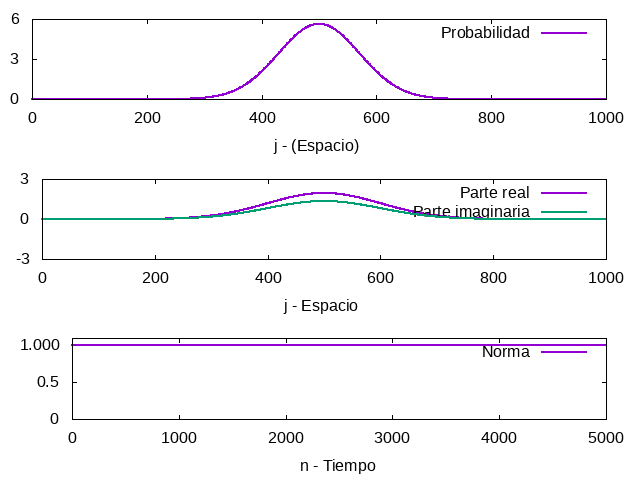
\includegraphics[width=0.485\textwidth]{Imagenes/N0PT1.png}}
    \subfigure[Función $\phi_0$ en $t_2$, $P(x,t)$ y la norma.]{
        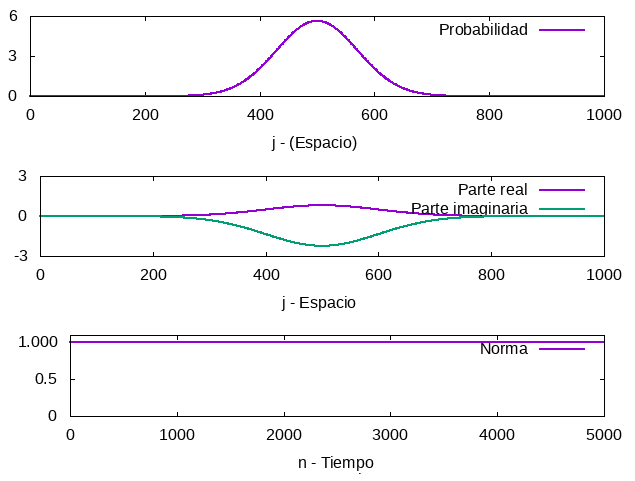
\includegraphics[width=0.485\textwidth]{Imagenes/N0PT2.png}}
    \subfigure[Función $\phi_0$ en $t_3$, $P(x,t)$ y la norma.]{
        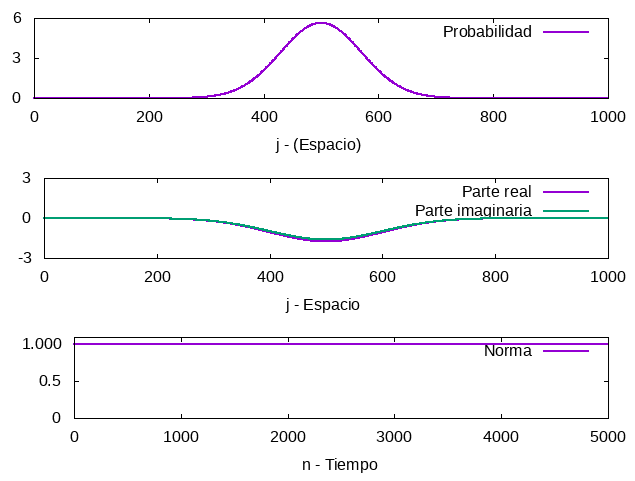
\includegraphics[width=0.485\textwidth]{Imagenes/N0PT3.png}}
    \subfigure[Valores de $<x(t)>$, $<p(t)>$ y $<H(t)>$.]{
        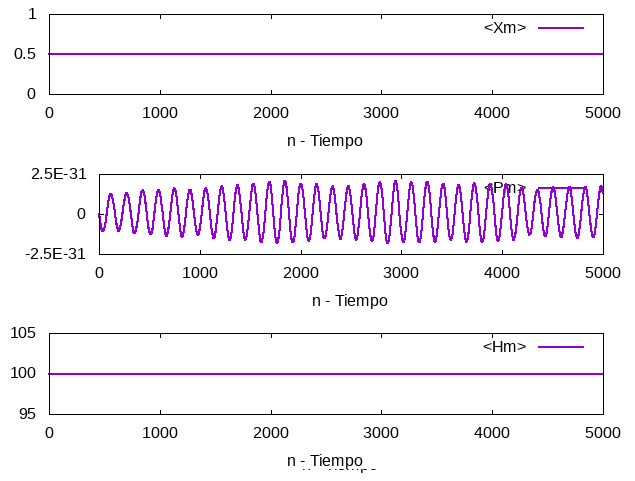
\includegraphics[width=0.49\textwidth]{Imagenes/N0O.png}}
    
  \end{center}
\end{figure}\\
\end{itemize}

\begin{itemize}
    \item N = 1.

\begin{figure}[H]
  \begin{center}

    \caption{Imágenes que representan las variaciones y desarrollo de la función de onda $\phi_1(x,t)$ a lo largo del tiempo según la ecuación de Schrödinger, junto a los valores de $P(x,t)$, la norma, $<x(t)>$, $<p(t)>$ y $<H(t)>$.}
    
    \subfigure[Función $\phi_1$ en $t_1$, $P(x,t)$ y la norma.]{
        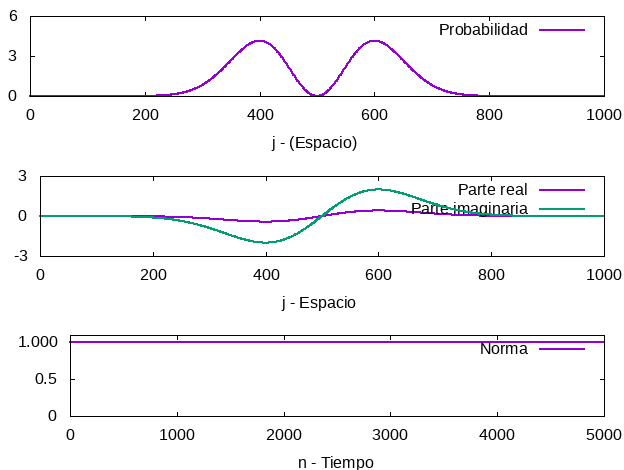
\includegraphics[width=0.485\textwidth]{Imagenes/N1PT1.png}}
    \subfigure[Función $\phi_1$ en $t_2$, $P(x,t)$ y la norma.]{
        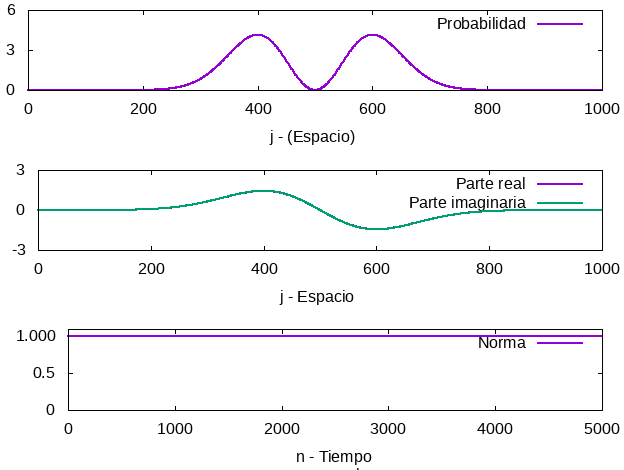
\includegraphics[width=0.485\textwidth]{Imagenes/N1PT2.png}}
    \subfigure[Función $\phi_1$ en $t_3$, $P(x,t)$ y la norma.]{
        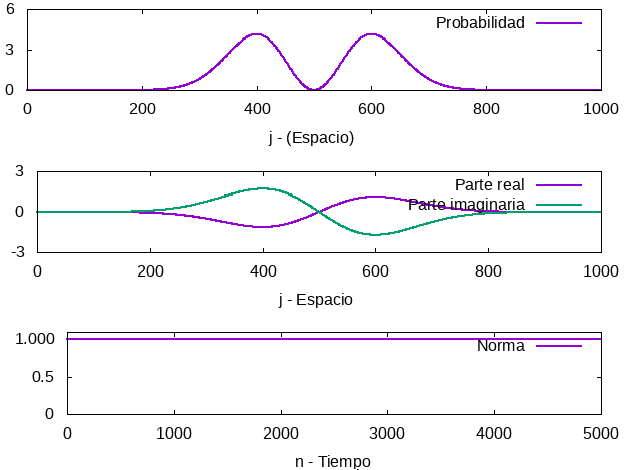
\includegraphics[width=0.485\textwidth]{Imagenes/N1PT3.png}}
    \subfigure[Valores de $<x(t)>$, $<p(t)>$ y $<H(t)>$.]{
        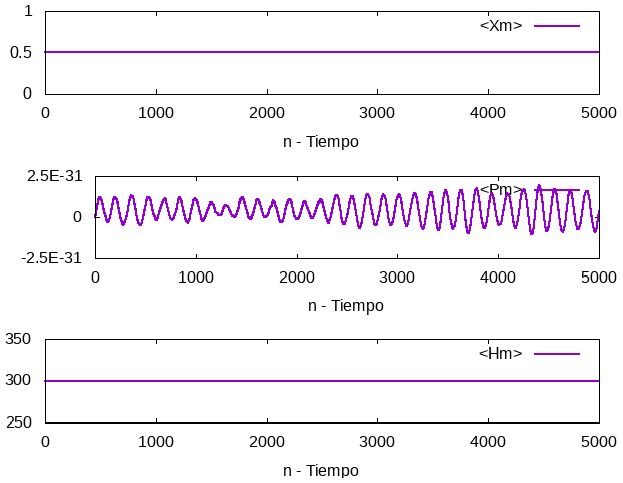
\includegraphics[width=0.485\textwidth]{Imagenes/N1O.png}}
    
  \end{center}
\end{figure}\\

\end{itemize}

\newpage
\begin{itemize}
    \item N = 2.
    \begin{figure}[H]
  \begin{center}

    \caption{Imágenes que representan las variaciones y desarrollo de la función de onda $\phi_2(x,t)$ a lo largo del tiempo según la ecuación de Schrödinger, junto a los valores de $P(x,t)$, la norma, $<x(t)>$, $<p(t)>$ y $<H(t)>$.}
    
    \subfigure[Función $\phi_2$ en $t_1$, $P(x,t)$ y la norma.]{
        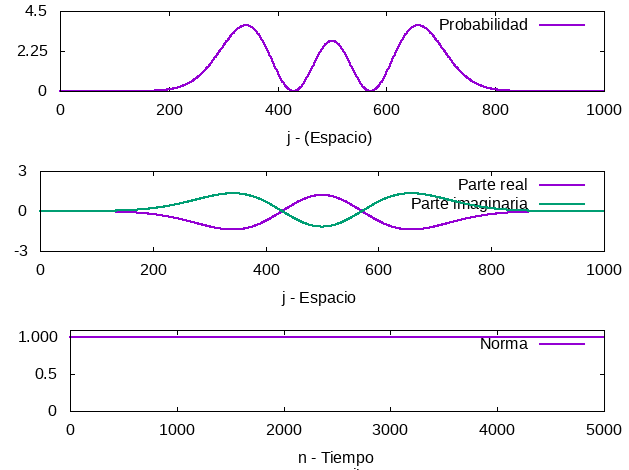
\includegraphics[width=0.485\textwidth]{Imagenes/N2PT1.png}}
    \subfigure[Función $\phi_2$ en $t_2$, $P(x,t)$ y la norma.]{
        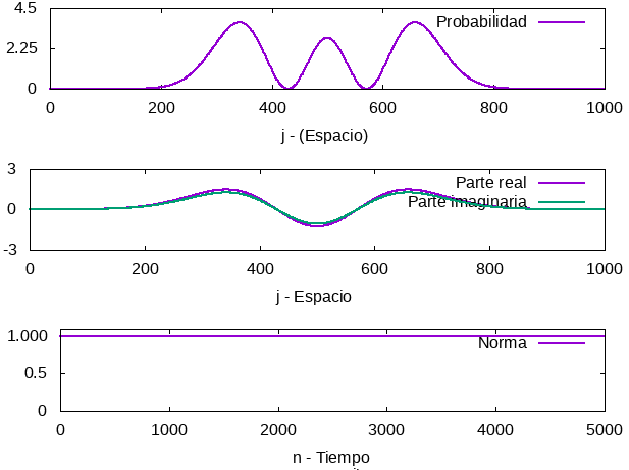
\includegraphics[width=0.485\textwidth]{Imagenes/N2PT2.png}}
    \subfigure[Función $\phi_2$ en $t_3$, $P(x,t)$ y la norma.]{
        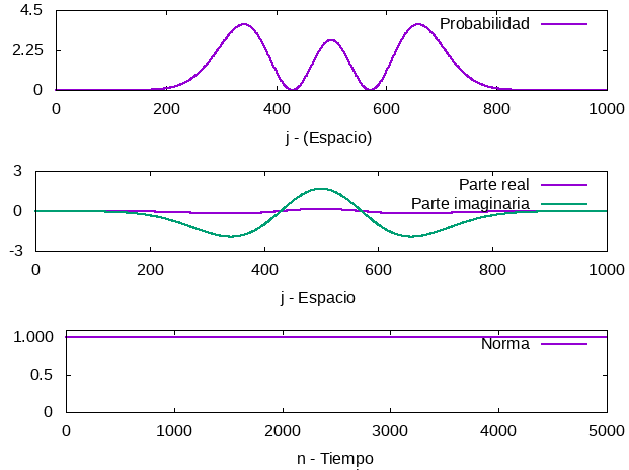
\includegraphics[width=0.485\textwidth]{Imagenes/N2PT3.png}}
    \subfigure[Valores de $<x(t)>$, $<p(t)>$ y $<H(t)>$.]{
        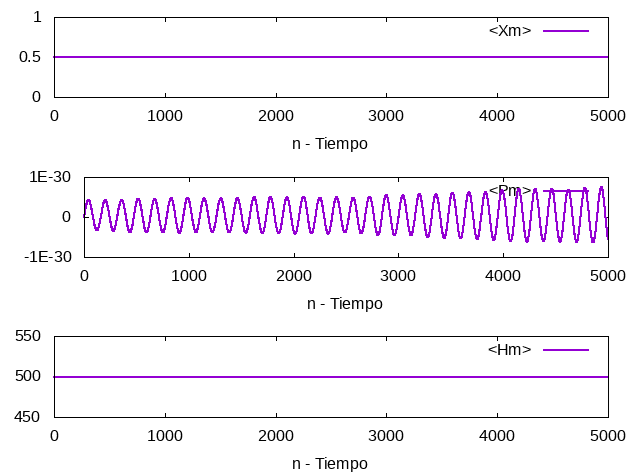
\includegraphics[width=0.485\textwidth]{Imagenes/N2O.png}}
    
  \end{center}
\end{figure}\\

\end{itemize}

\newpage
\begin{itemize}
    \item N = 3.
    \begin{figure}[H]
  \begin{center}

    \caption{Imágenes que representan las variaciones y desarrollo de la función de onda $\phi_3(x,t)$ a lo largo del tiempo según la ecuación de Schrödinger, junto a los valores de $P(x,t)$, la norma, $<x(t)>$, $<p(t)>$ y $<H(t)>$.}
    
    \subfigure[Función $\phi_3$ en $t_1$, $P(x,t)$ y la norma.]{
        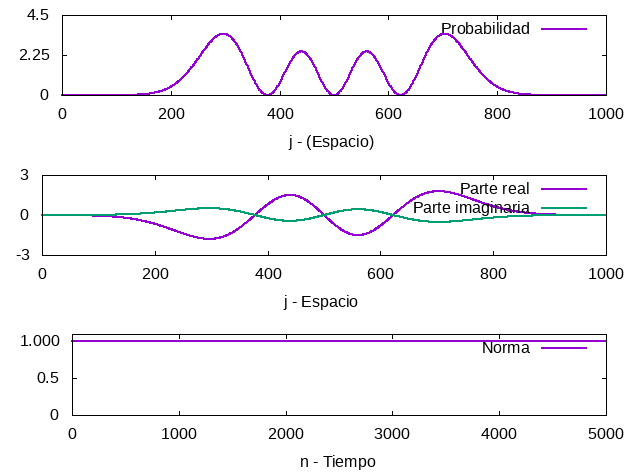
\includegraphics[width=0.485\textwidth]{Imagenes/N3PT1.png}}
    \subfigure[Función $\phi_3$ en $t_2$, $P(x,t)$ y la norma.]{
        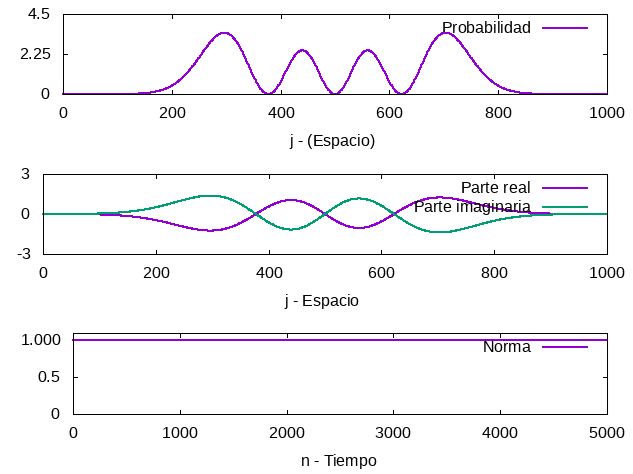
\includegraphics[width=0.485\textwidth]{Imagenes/N3PT2.png}}
    \subfigure[Función $\phi_3$ en $t_3$, $P(x,t)$ y la norma.]{
        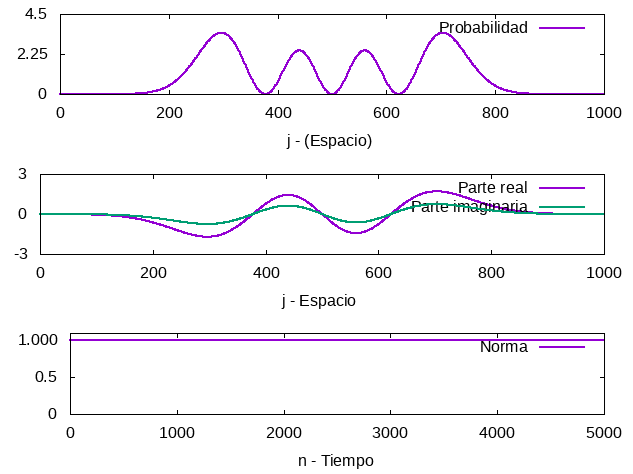
\includegraphics[width=0.485\textwidth]{Imagenes/N3PT3.png}}
    \subfigure[Valores de $<x(t)>$, $<p(t)>$ y $<H(t)>$.]{
        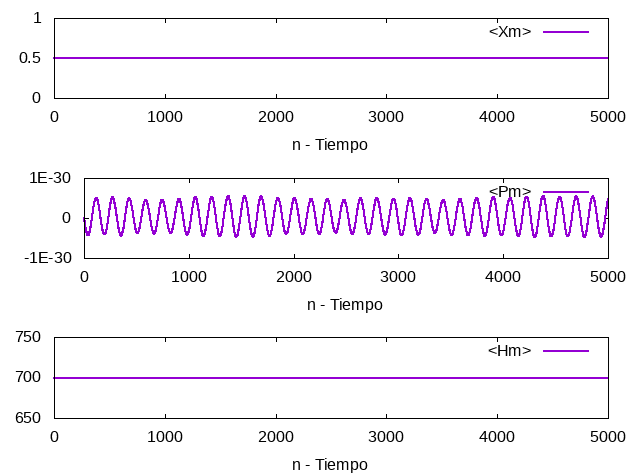
\includegraphics[width=0.485\textwidth]{Imagenes/N3O.png}}
    
  \end{center}
\end{figure}\\

\end{itemize}
Primero cabe resaltar cómo va aumentando el número de vientres en las ondas según aumentas el número cuántico, siendo N+1 vientres para un número cuántico N, y por consiguiente el aumento de la densidad de probabilidad, encontrando que es mucho mayor de encontrar las partículas en posiciones muy diferentes para cada número cuántico. Cabe resaltar que la norma en todo momento se mantiene constante y entorno a 1, pues se ha realizado la ecuación de Schrödinger para una función normalizada. Cómo la posición media de la partícula sea cual sea el caso se mantiene constante, justo donde la hemos definido, en $x_0 = 0.5$. Y cómo las variaciones en la amplitud del momento medio son mayores conforme aumenta N, lo que explica el correspondiente aumento de la energía media. Esto es fácilmente explicable si visualizamos la ecuación de la función de onda, pues para mayores N, mayor será el exponente de la función, y por tanto al realizar los valores medios, es normal que salgan valores mucho mayores.\\

\newpage
\begin{itemize}
    \item $\Delta x \Delta p$ para $N=0$ y $N=1$:
    \begin{figure}[H]
  \begin{center}

    \caption{Imágenes que representan las variaciones y desarrollo de $\Delta x \Delta p$ a lo largo del tiempo para $N=0$ y $N=1$.}
    
    \subfigure[$\Delta x \Delta p$ para la función $\phi_0$.]{
        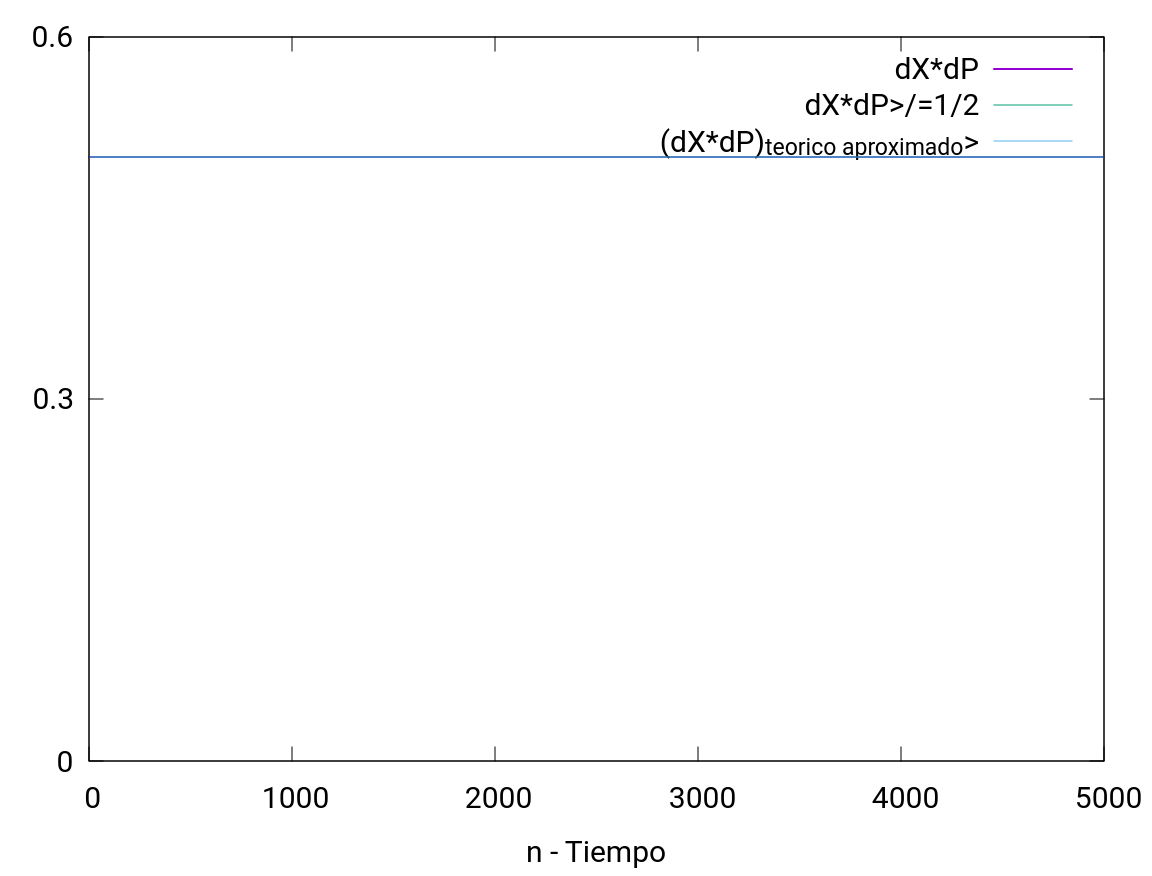
\includegraphics[width=0.725\textwidth]{Imagenes/PHeiN0.png}}
    \subfigure[\textbf{Función $\phi_1$ en $t_2$, $P(x,t)$ y la norma.}]{
        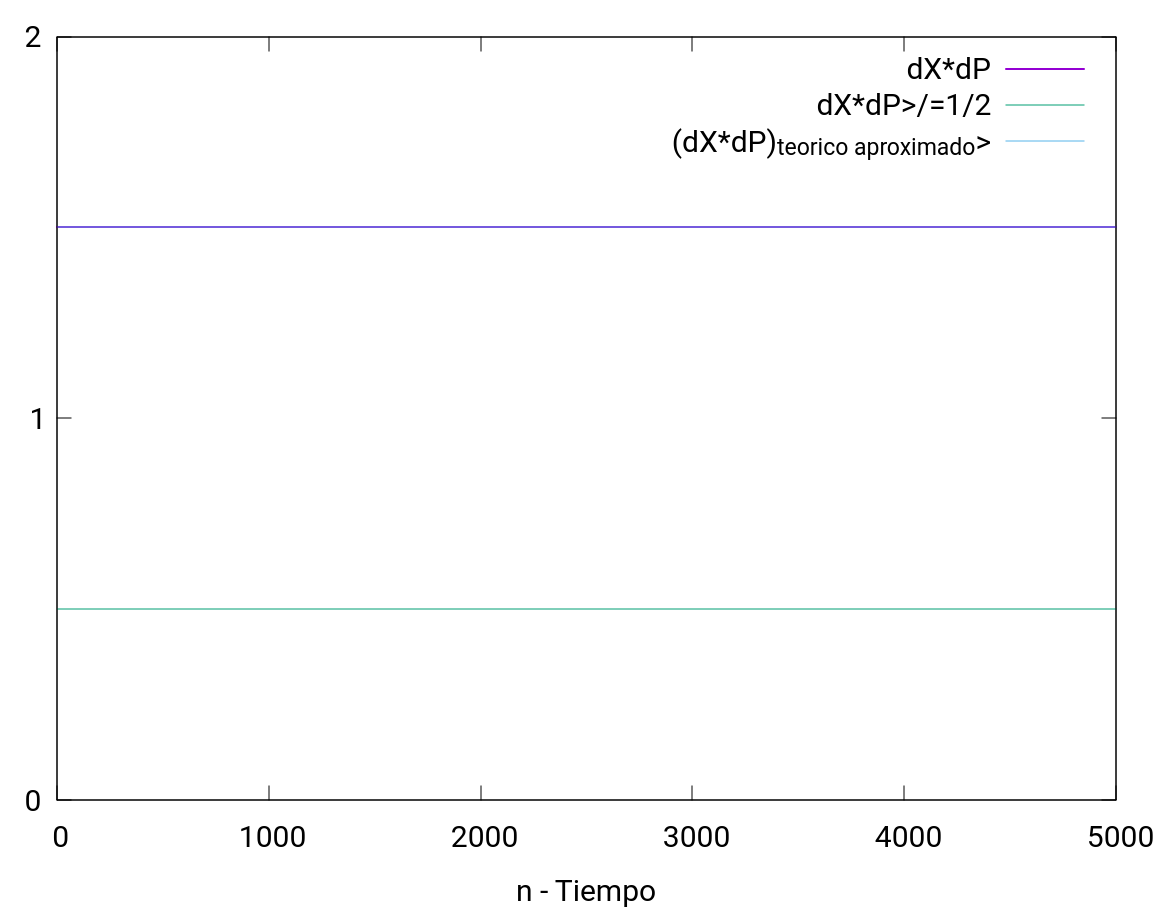
\includegraphics[width=0.725\textwidth]{Imagenes/PHeiN1.png}}

  \end{center}
\end{figure}\\
\end{itemize}
En donde podemos comprobar que los valores teóricos se ajustan completamente a los obtenidos computacionalmente, en ambos casos cumplen el principio de Heisenberg.

\newpage
\subsubsection{Función Gaussiana.}

\begin{itemize}
    \item Caso 1.

\begin{figure}[H]
  \begin{center}

    \caption{Imágenes que representan las variaciones y desarrollo de la función de onda $\phi(x,t)$ Gaussiana para el caso 1 a lo largo del tiempo según la ecuación de Schrödinger, junto a los valores de $P(x,t)$, la norma, $<x(t)>$, $<p(t)>$ y $<H(t)>$.}
    
    \subfigure[Función $\phi$ Gaussiana en $t_1$, $P(x,t)$ y la norma.]{
        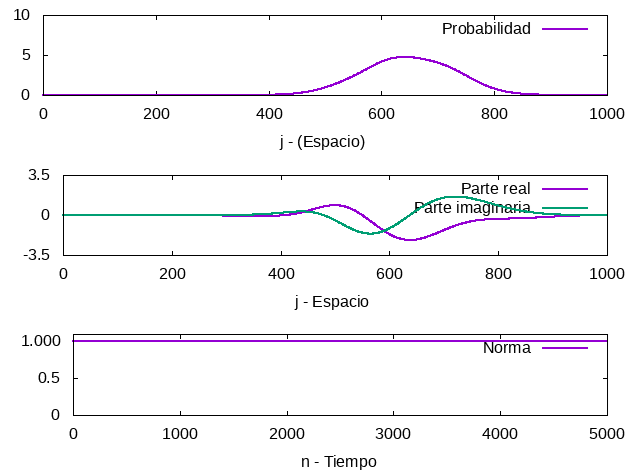
\includegraphics[width=0.485\textwidth]{Imagenes/G1PT1.png}}
    \subfigure[Función $\phi$ Gaussiana en $t_2$, $P(x,t)$ y la norma.]{
        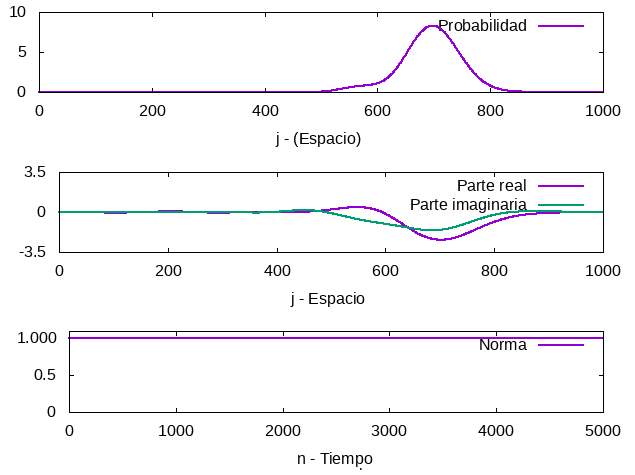
\includegraphics[width=0.485\textwidth]{Imagenes/G1PT2.png}}
    \subfigure[Función $\phi$ Gaussiana en $t_3$, $P(x,t)$ y la norma.]{
        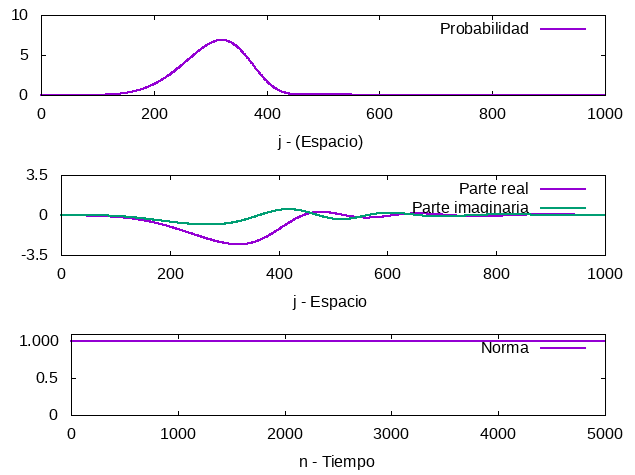
\includegraphics[width=0.485\textwidth]{Imagenes/G1PT3.png}}
        \subfigure[Función $\phi$ Gaussiana en $t_4$, $P(x,t)$ y la norma.]{
        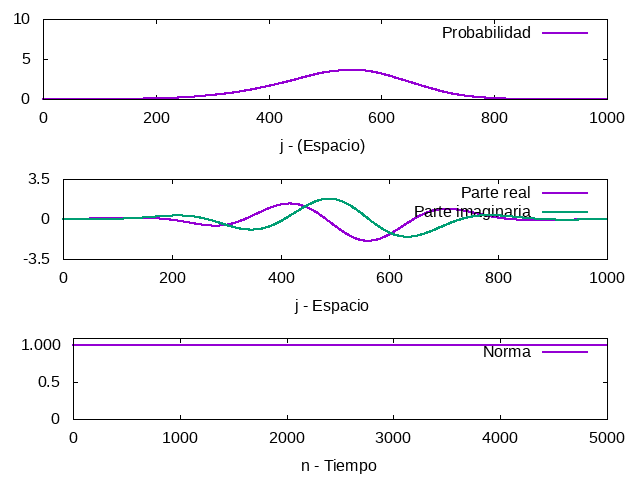
\includegraphics[width=0.485\textwidth]{Imagenes/G1PT4.png}}
    \subfigure[Valores de $<x(t)>$, $<p(t)>$ y $<H(t)>$.]{
        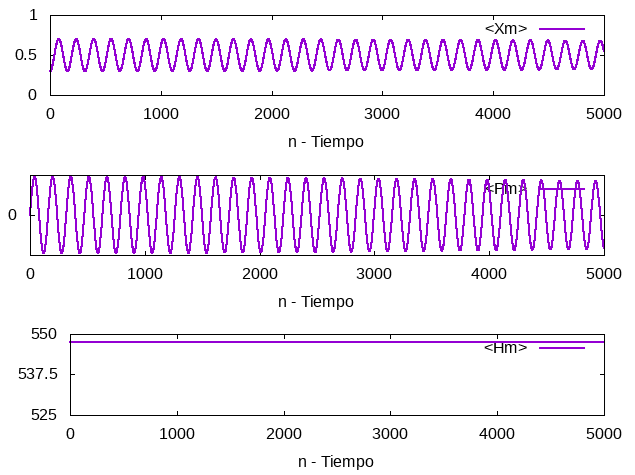
\includegraphics[width=0.485\textwidth]{Imagenes/G1O.png}}
    
  \end{center}
\end{figure}\\

\end{itemize}

\begin{itemize}
    \item Caso 2.

\begin{figure}[H]
  \begin{center}

    \caption{Imágenes que representan las variaciones y desarrollo de la función de onda $\phi(x,t)$ Gaussiana para el caso 2 a lo largo del tiempo según la ecuación de Schrödinger, junto a los valores de $P(x,t)$, la norma, $<x(t)>$, $<p(t)>$ y $<H(t)>$.}
    
    \subfigure[Función $\phi$ Gaussiana en $t_1$, $P(x,t)$ y la norma.]{
        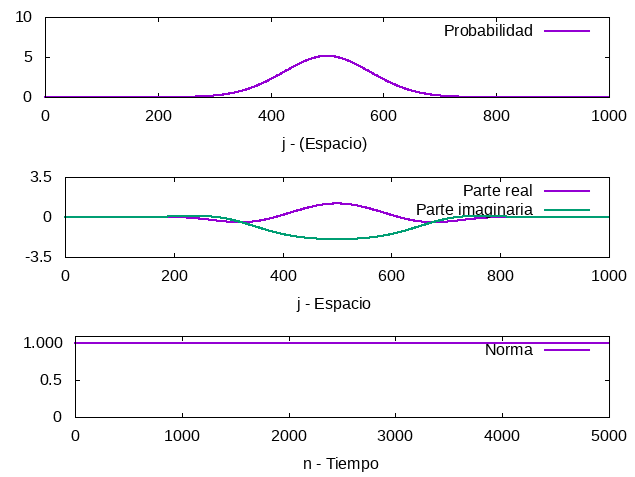
\includegraphics[width=0.485\textwidth]{Imagenes/G2PT1.png}}
    \subfigure[Función $\phi$ Gaussiana en $t_2$, $P(x,t)$ y la norma.]{
        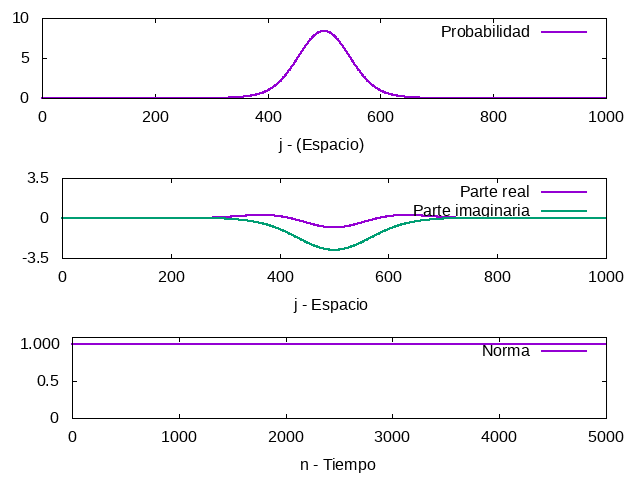
\includegraphics[width=0.485\textwidth]{Imagenes/G2PT2.png}}
    \subfigure[Función $\phi$ Gaussiana en $t_3$, $P(x,t)$ y la norma.]{
        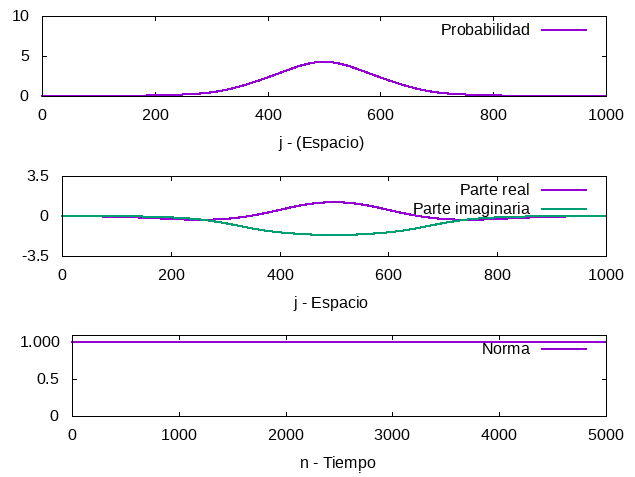
\includegraphics[width=0.485\textwidth]{Imagenes/G2PT3.png}}
        \subfigure[Función $\phi$ Gaussiana en $t_4$, $P(x,t)$ y la norma.]{
        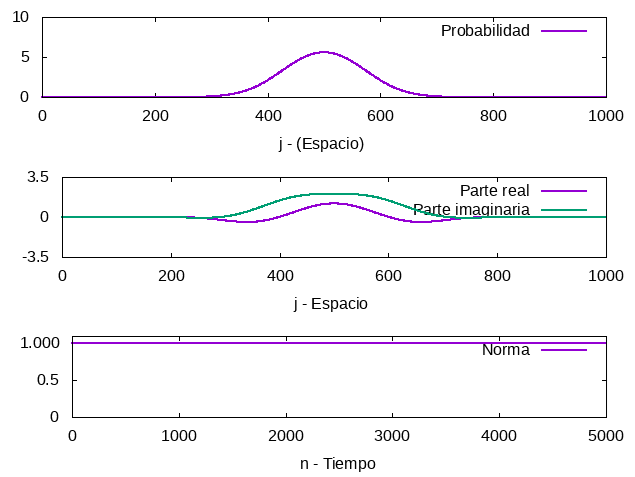
\includegraphics[width=0.485\textwidth]{Imagenes/G2PT4.png}}
    \subfigure[Valores de $<x(t)>$, $<p(t)>$ y $<H(t)>$.]{
        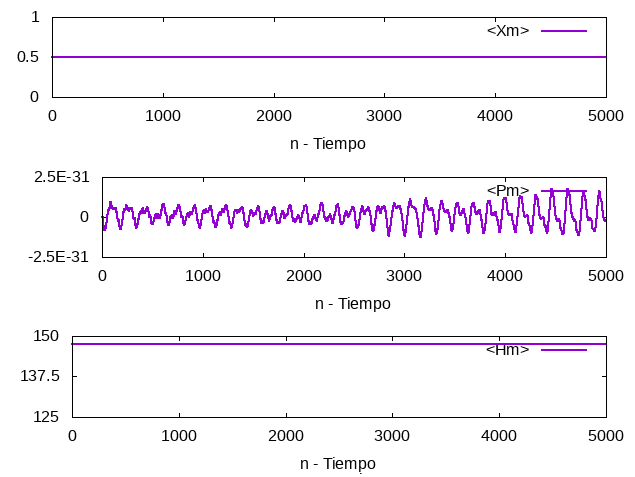
\includegraphics[width=0.485\textwidth]{Imagenes/G2O.png}}
    
  \end{center}
\end{figure}\\

\end{itemize}

\newpage
\begin{itemize}
    \item Caso 3.

\begin{figure}[H]
  \begin{center}

    \caption{Imágenes que representan las variaciones y desarrollo de la función de onda $\phi(x,t)$ Gaussiana para el caso 3 a lo largo del tiempo según la ecuación de Schrödinger, junto a los valores de $P(x,t)$, la norma, $<x(t)>$, $<p(t)>$ y $<H(t)>$.}
    
    \subfigure[Función $\phi$ Gaussiana en $t_1$, $P(x,t)$ y la norma.]{
        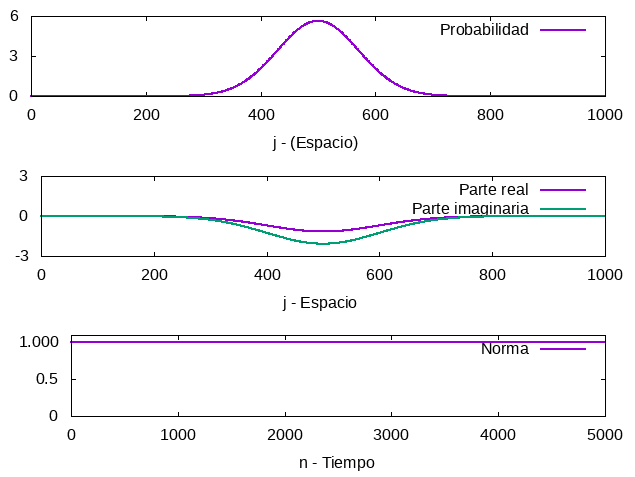
\includegraphics[width=0.485\textwidth]{Imagenes/G3PT1.png}}
    \subfigure[Función $\phi$ Gaussiana en $t_2$, $P(x,t)$ y la norma.]{
        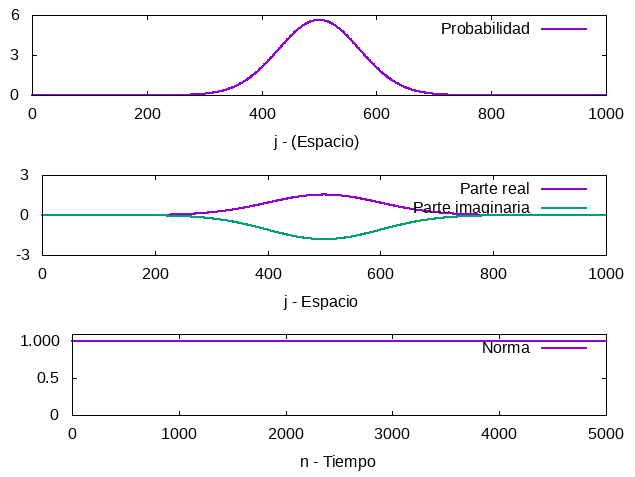
\includegraphics[width=0.485\textwidth]{Imagenes/G3PT2.png}}
    \subfigure[Función $\phi$ Gaussiana en $t_3$, $P(x,t)$ y la norma.]{
        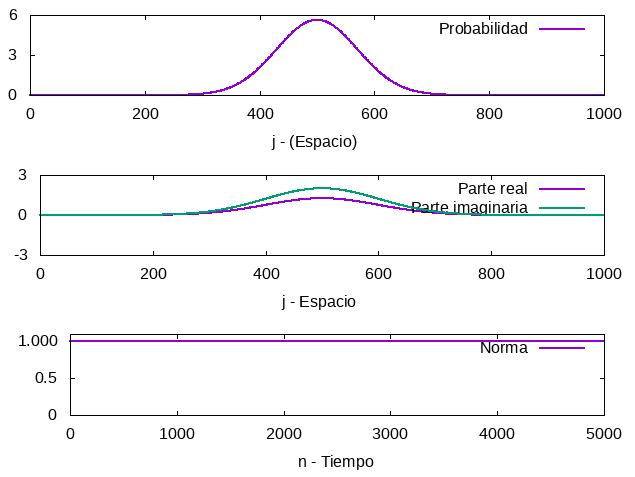
\includegraphics[width=0.485\textwidth]{Imagenes/G3PT3.png}}
    \subfigure[Valores de $<x(t)>$, $<p(t)>$ y $<H(t)>$.]{
        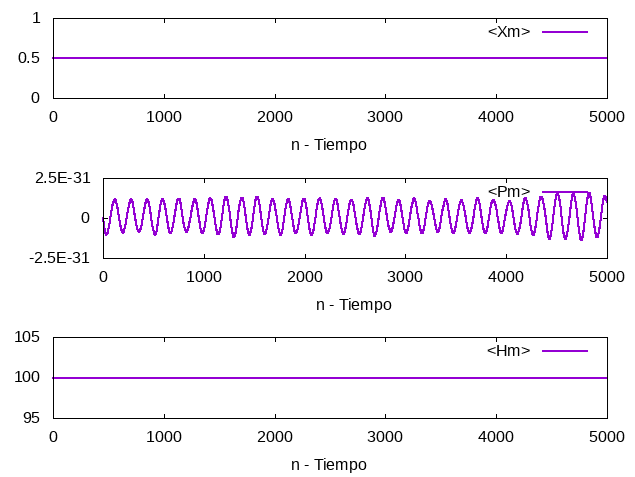
\includegraphics[width=0.485\textwidth]{Imagenes/G3O.png}}
    
  \end{center}
\end{figure}\\
\end{itemize}
Podemos comprobar con bastante claridad lo anteriormente expuesto. En el primer caso el potencial produce que la onda tenga un cambio de posición de lado a lado de la caja, produciendo cambios en la densidad de probabilidad y variándola completamente de lugar. Dicho movimiento es periódico y cómo tal podemos verlo reflejado en los valores de la posición media. Para el segundo caso vemos una densidad de probabilidad prácticamente fija en el espacio pero con variancias en su tamaño a lo largo del tiempo, podemos ver que dichas variaciones pueden ser debidas al potencial que hace variar la función de onda centrada en en el punto $x_0$. En este caso la posición media se mantiene constante, logicamente. Y finalmente, el último caso es exactamente igual que el caso en el que N=1. Esto lo podemos ver más claramente reflejado en las variaciones de $\Delta x \Delta p $, donde denotamos valores variables para los 2 primeros casos y valores exactos para N=0 para el tercer caso:
\begin{figure}[H]
  \begin{center}

    \caption{Imágenes que representan las variaciones y desarrollo de $\Delta x \Delta p$ a lo largo del tiempo para los 3 diferentes casos.}
    
    \subfigure[$\Delta x \Delta p$ para la función $\phi$ Gaussiana para el caso 1.]{
        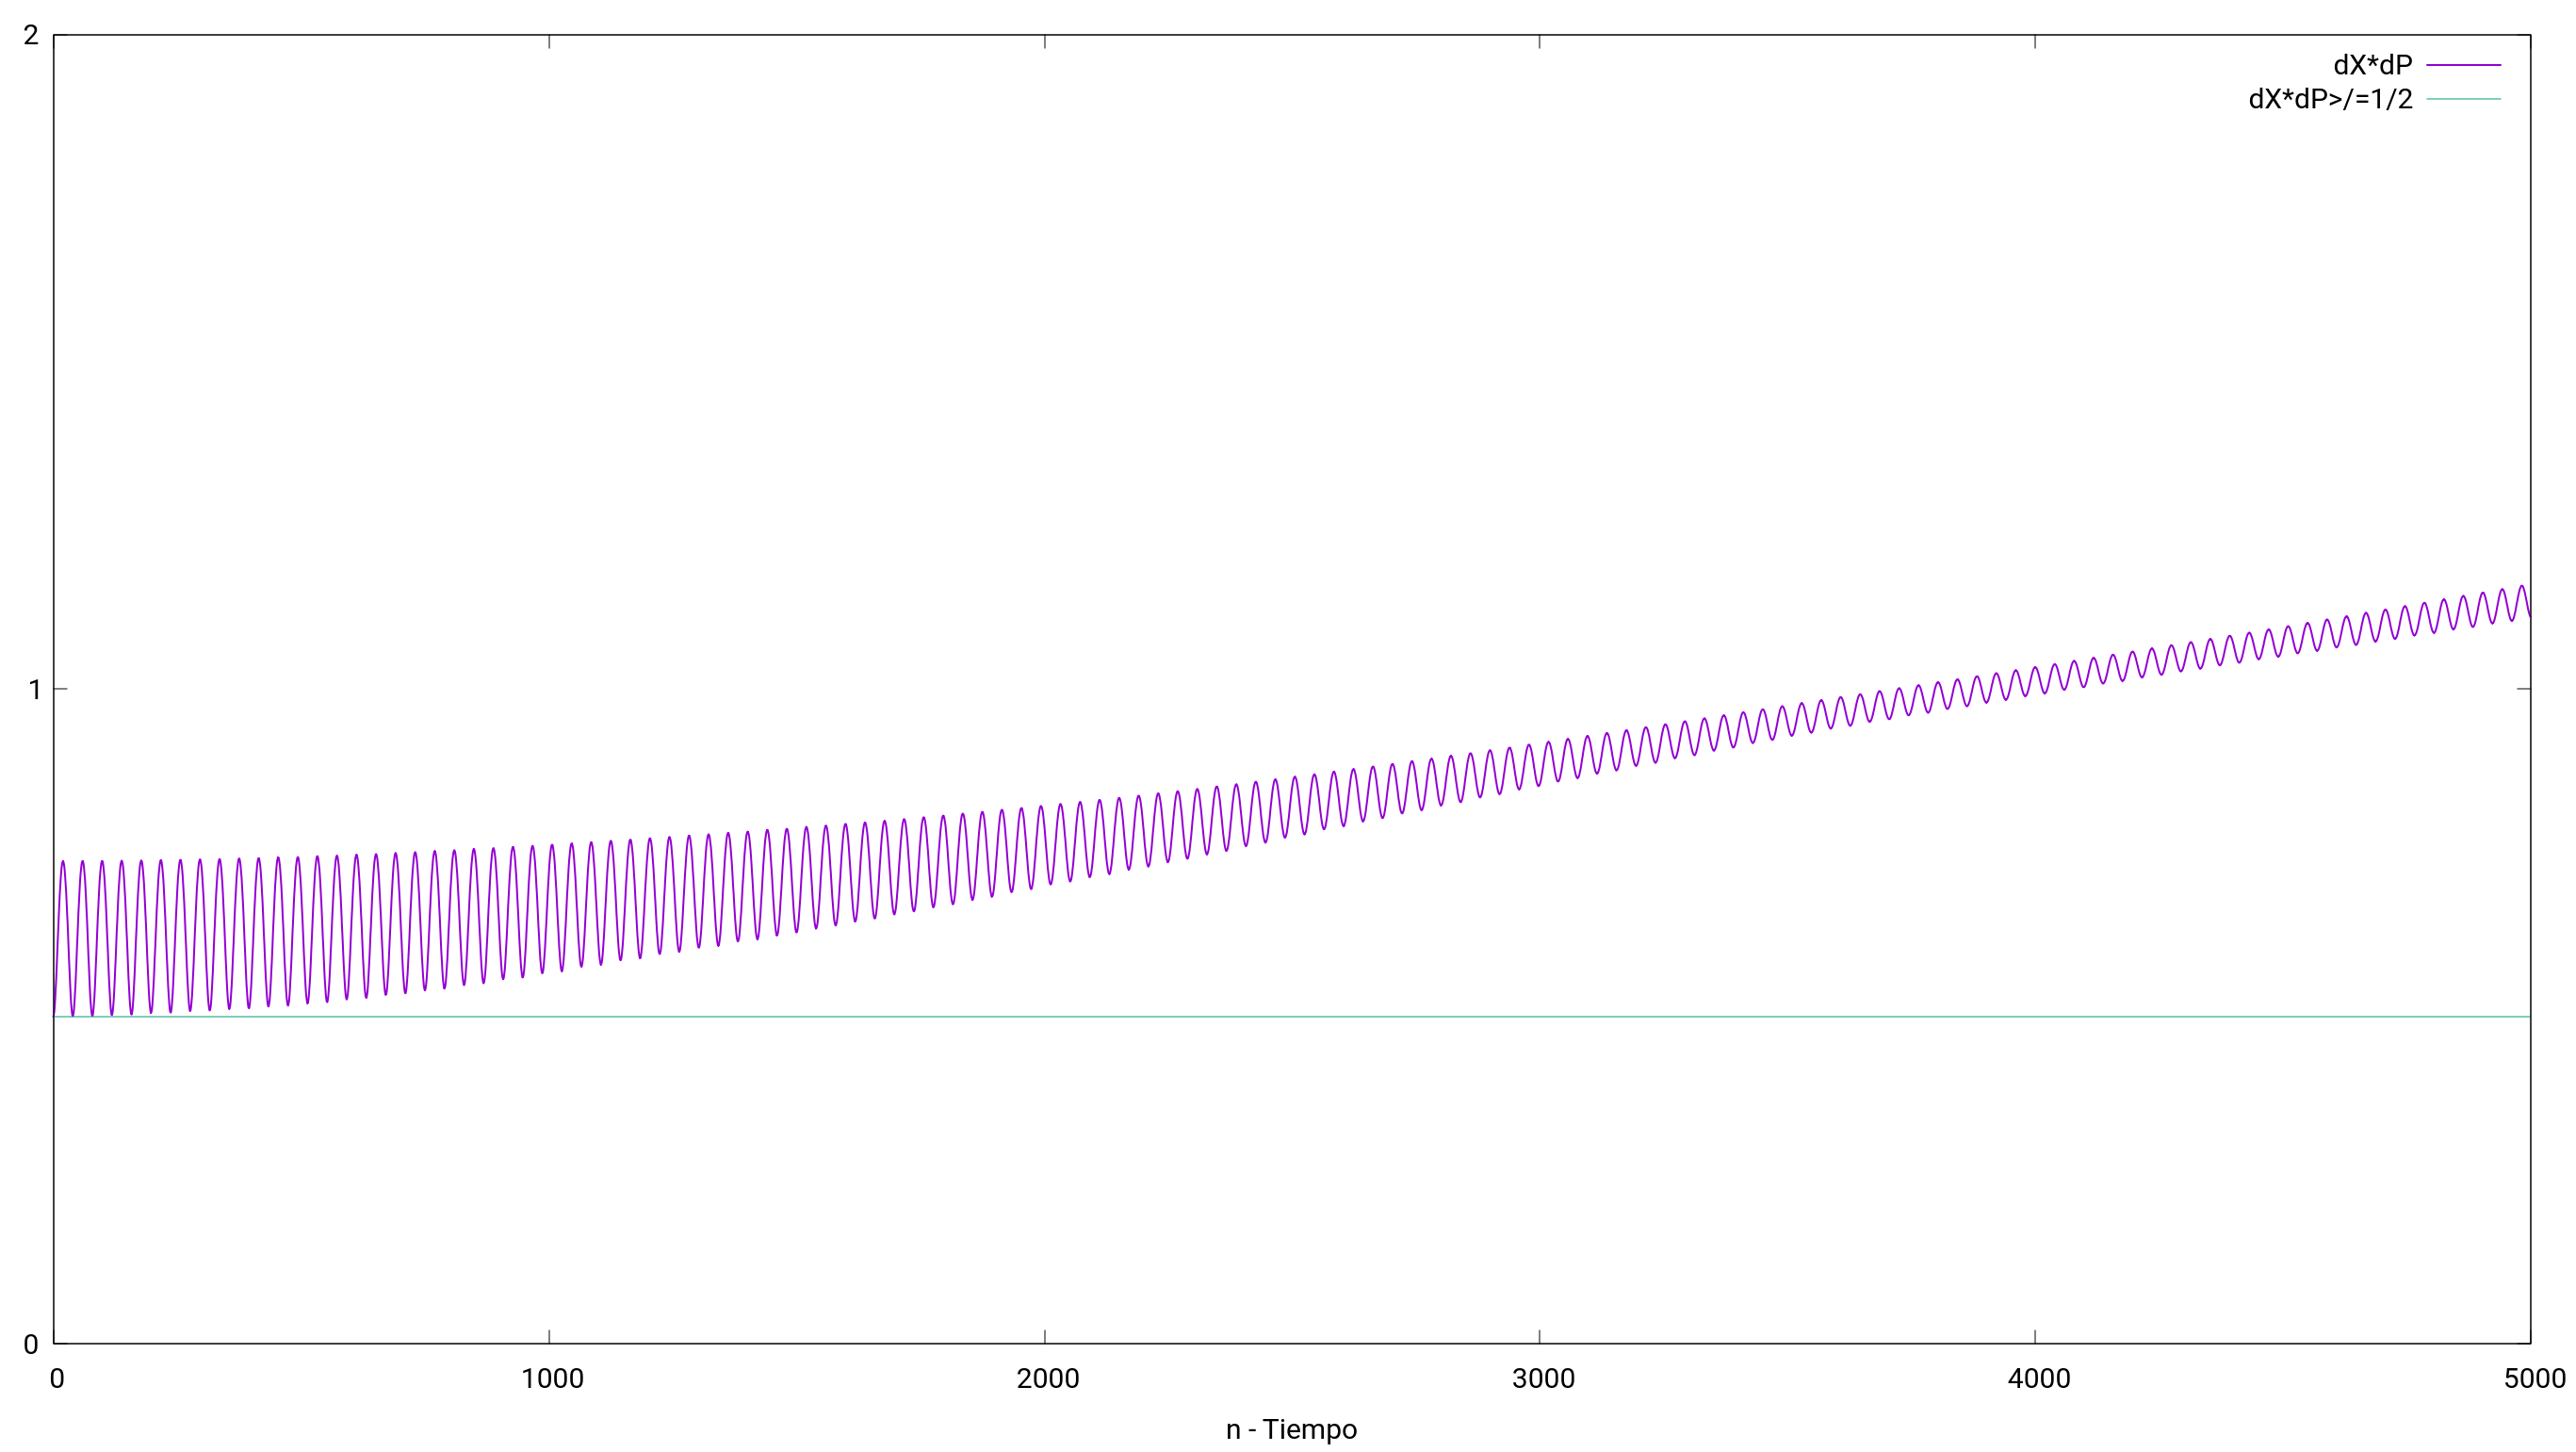
\includegraphics[width=0.725\textwidth]{Imagenes/PHeiG1.png}}
    \subfigure[$\Delta x \Delta p$ para la función $\phi$ Gaussiana para el caso 2.]{
        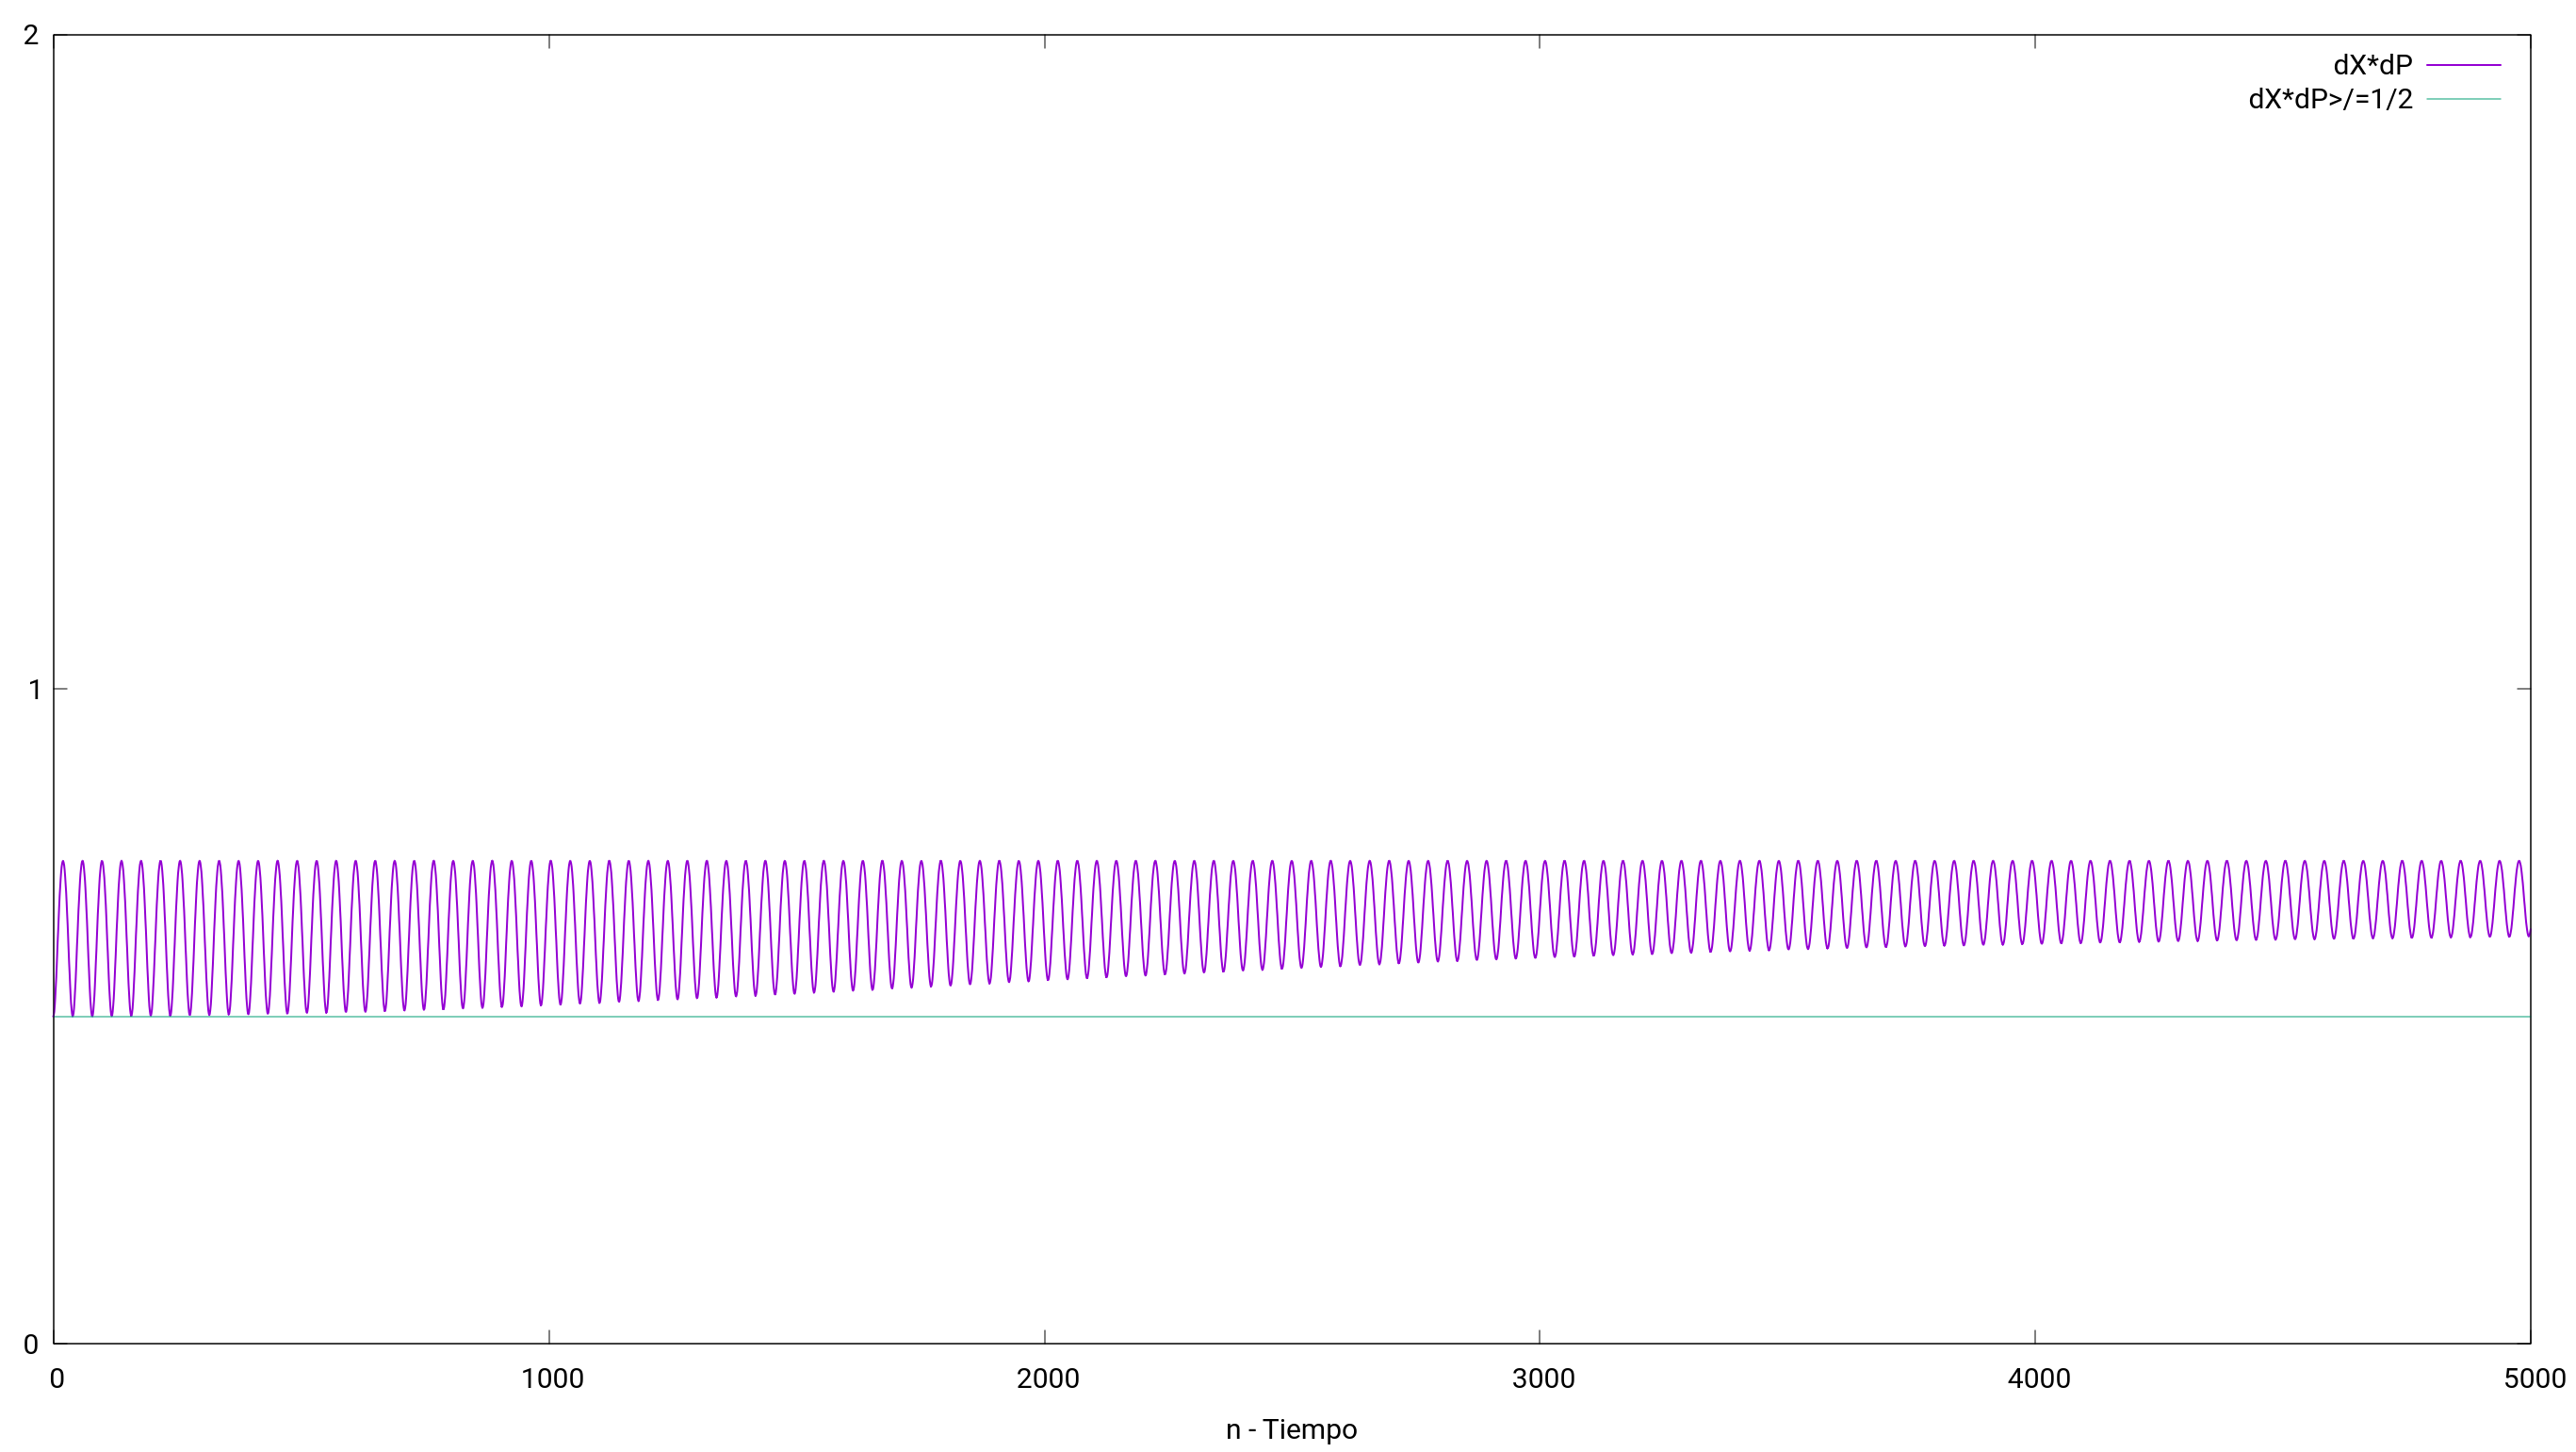
\includegraphics[width=0.725\textwidth]{Imagenes/PHeiG2.png}}
    \subfigure[$\Delta x \Delta p$ para la función $\phi$ Gaussiana para el caso 3.]{
        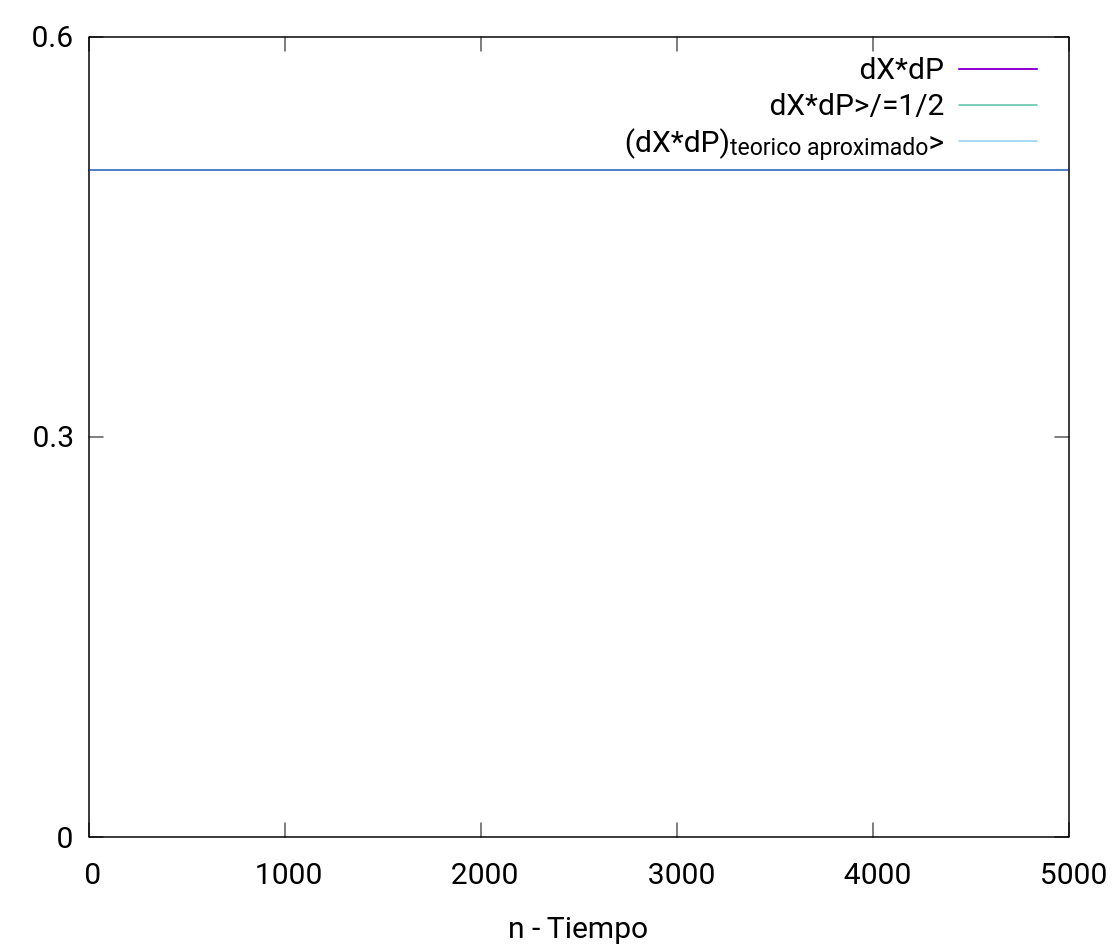
\includegraphics[width=0.6\textwidth]{Imagenes/PHeiG3.png}}

  \end{center}
\end{figure}\\
\subsubsection{Comparación probabilidad clásica con la cuántico.}
Para el cálculo de la probabilidad clásica se ha hecho uso de la siguiente ecuación dada en el capítulo 4 de Introduction to quantum mechanics de B.H. Bransden y C.J. Joachin:
\begin{equation*}
    P_C(\xi) = \frac{1}{\pi (\xi_0^2-\xi^2)}
\end{equation*}
Y se ha hecho un ajuste de la probabilidad tal que: $P(x,t)/\alpha$ para todas las gráficas.
\begin{figure}[H]
  \begin{center}

    \caption{Imágenes que representan las variaciones y desarrollo de $P(x,t)$ (color violáceo) y de $P_C$ (color verdoso) para diferentes N (0 y 5).}
    
    \subfigure[$P(x,t)$ para N=0 comparado con $P_C$.]{
        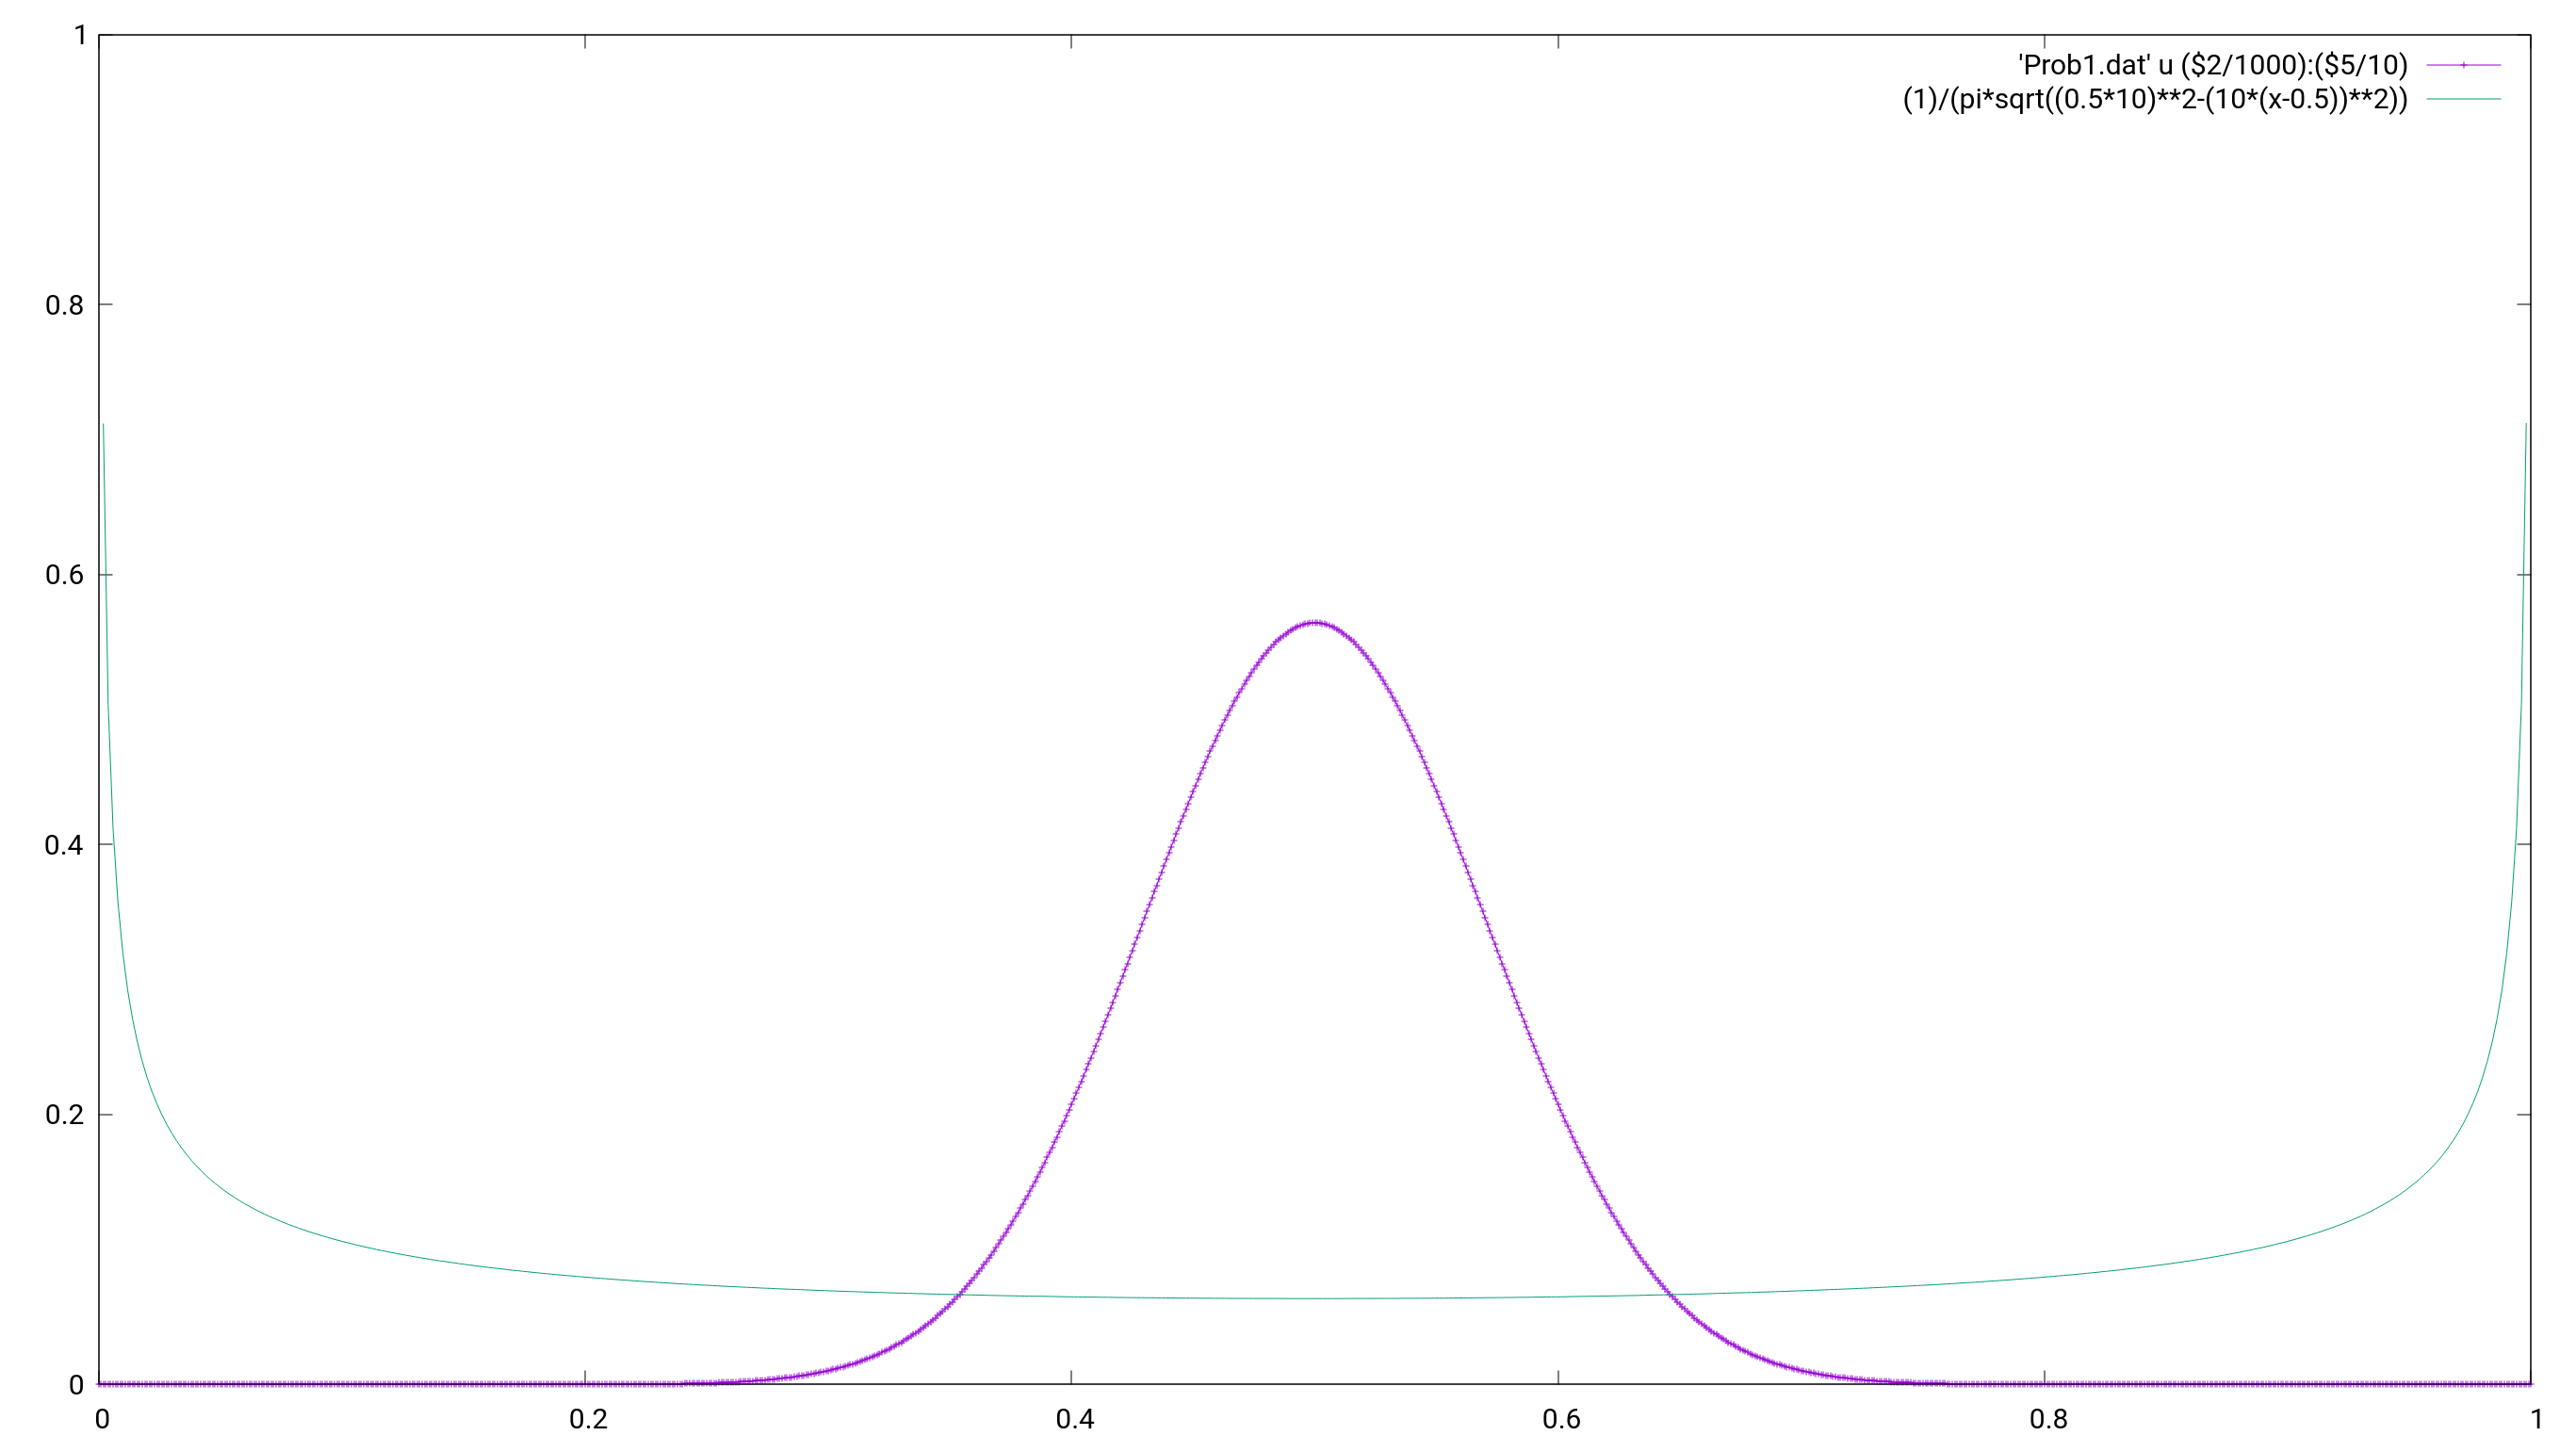
\includegraphics[width=0.825\textwidth]{Imagenes/ComPcyParmN0.png}}
    \subfigure[$P(x,t)$ para N=5 comparado con $P_C$.]{
        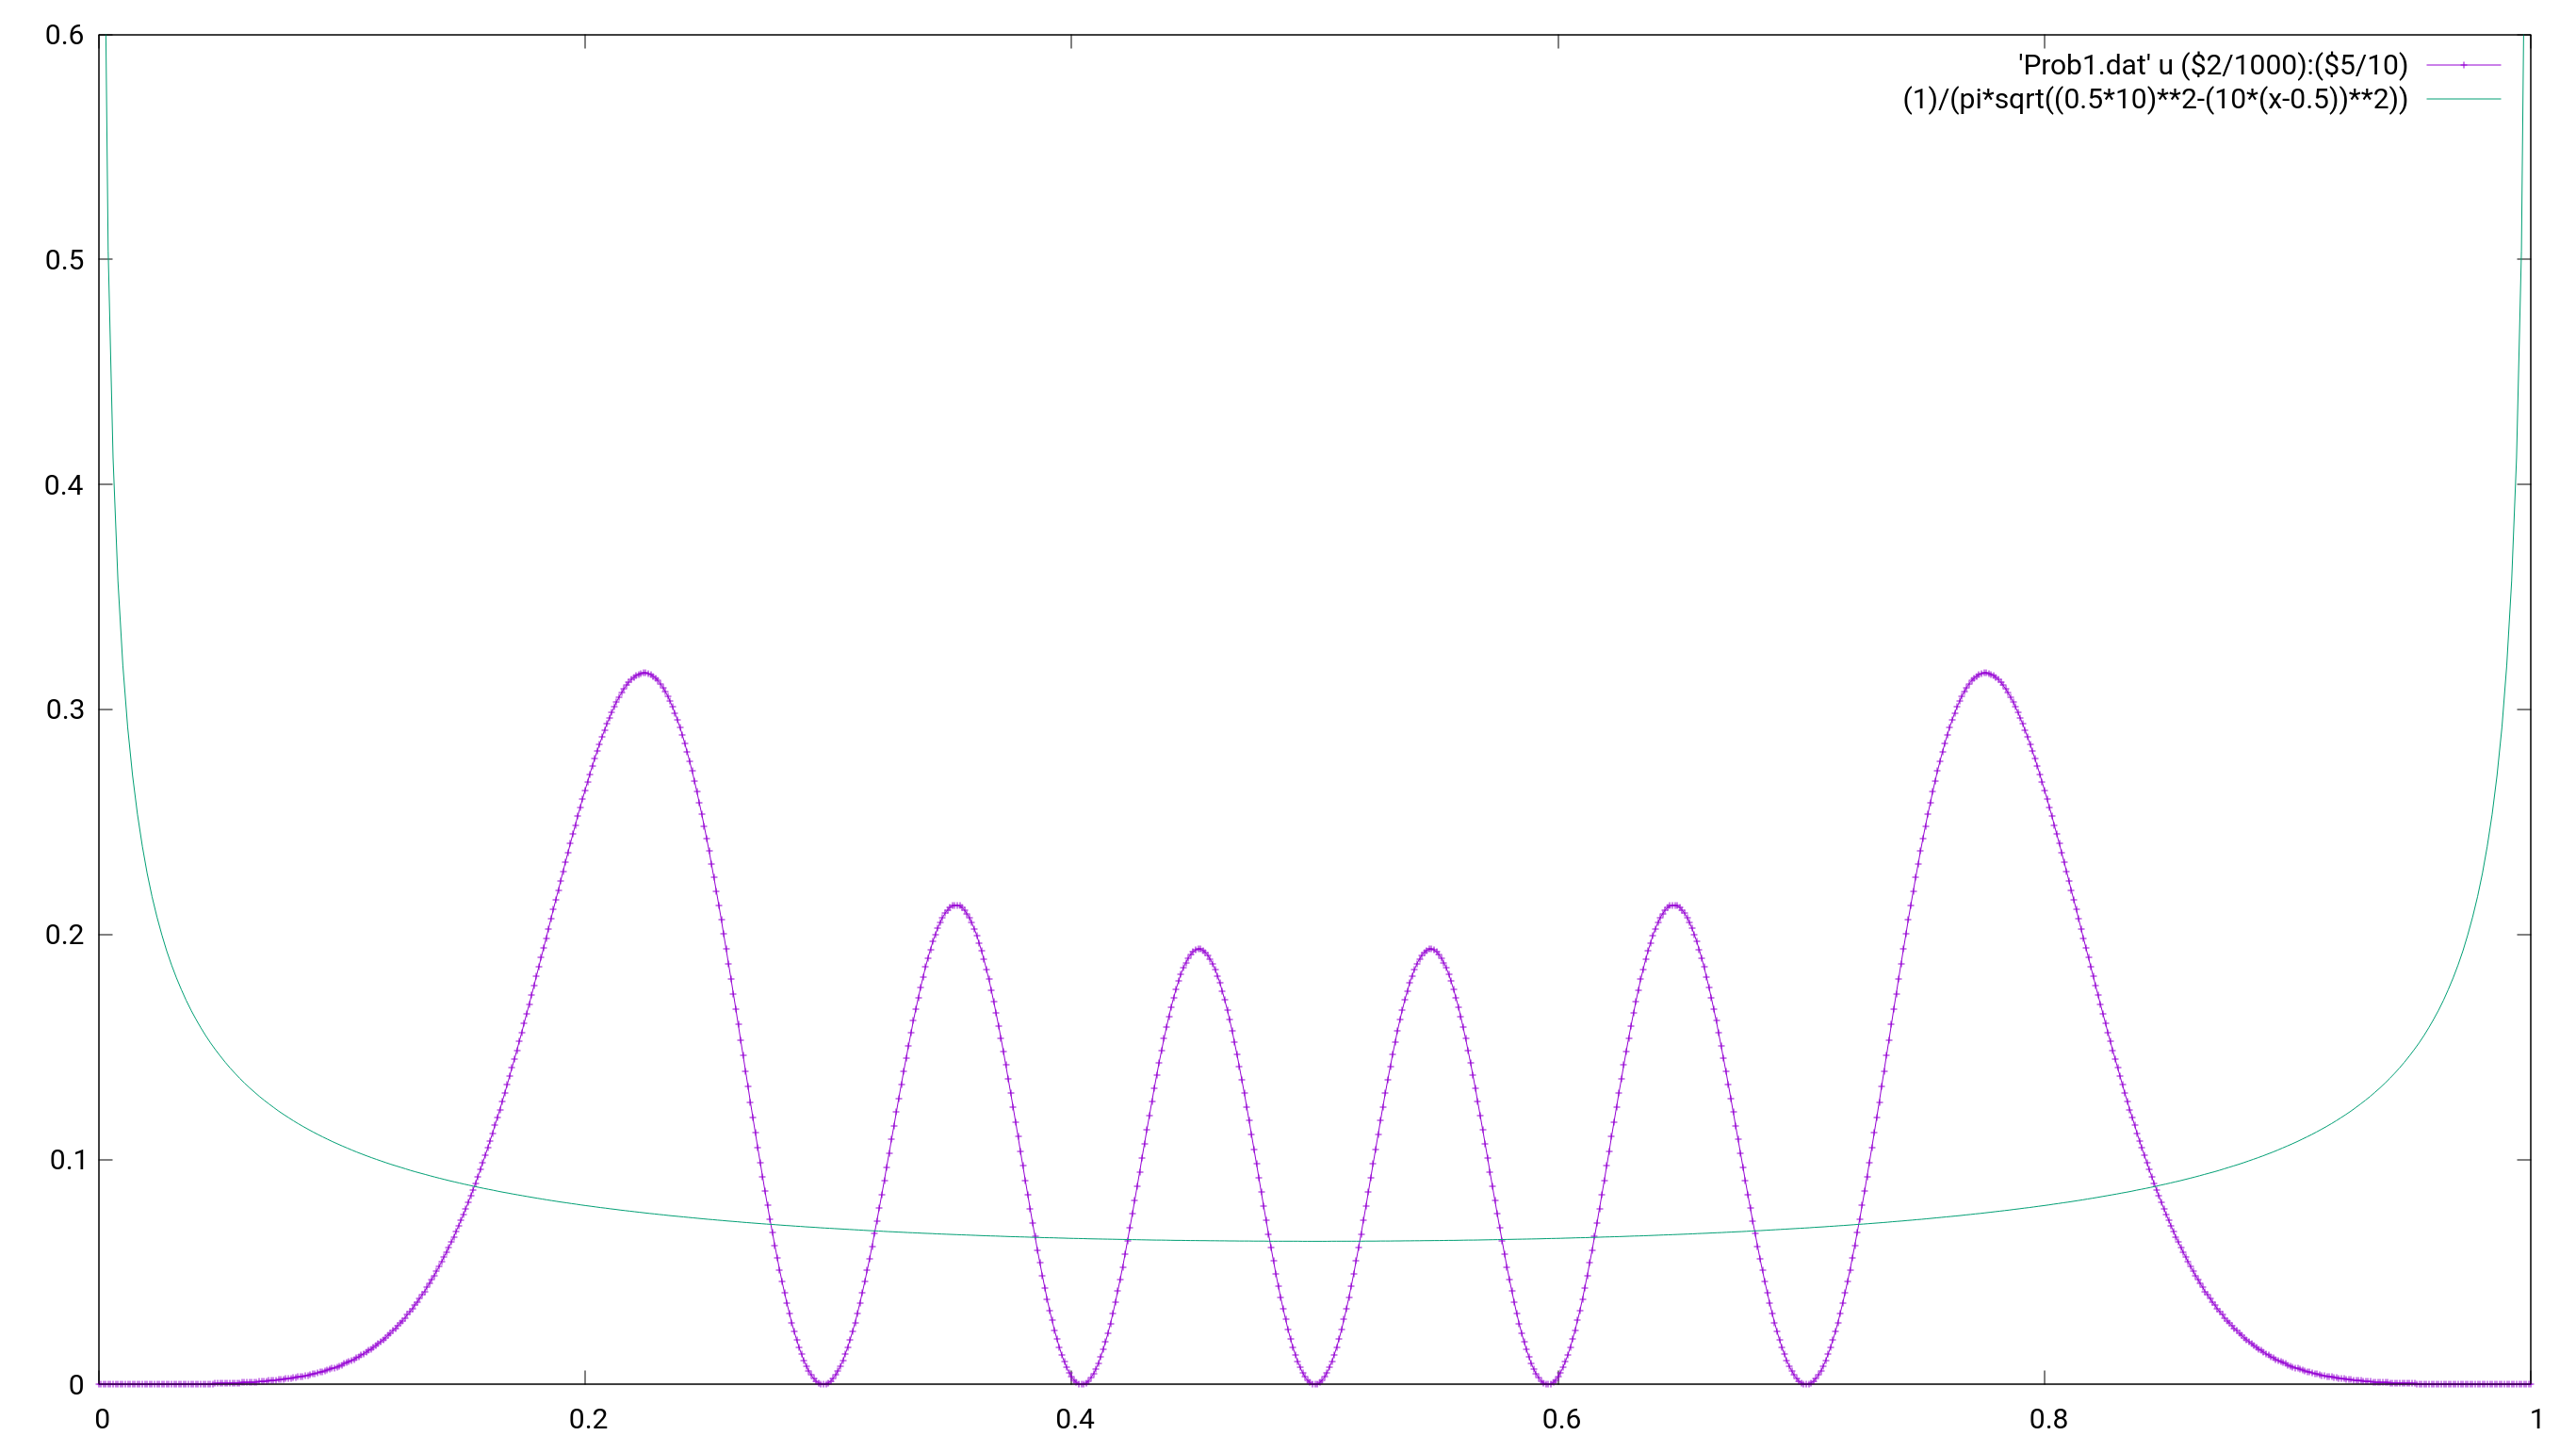
\includegraphics[width=0.825\textwidth]{Imagenes/ComPcyParmN5.png}}
    

  \end{center}
\end{figure}\\
\newpage
\begin{figure}[H]
  \begin{center}

    \caption{Imágenes que representan las variaciones y desarrollo de $P(x,t)$ (color violáceo) y de $P_C$ (color verdoso) para diferentes N (10, 15 y 20).}
    \subfigure[$P(x,t)$ para N=10 comparado con $P_C$.]{
        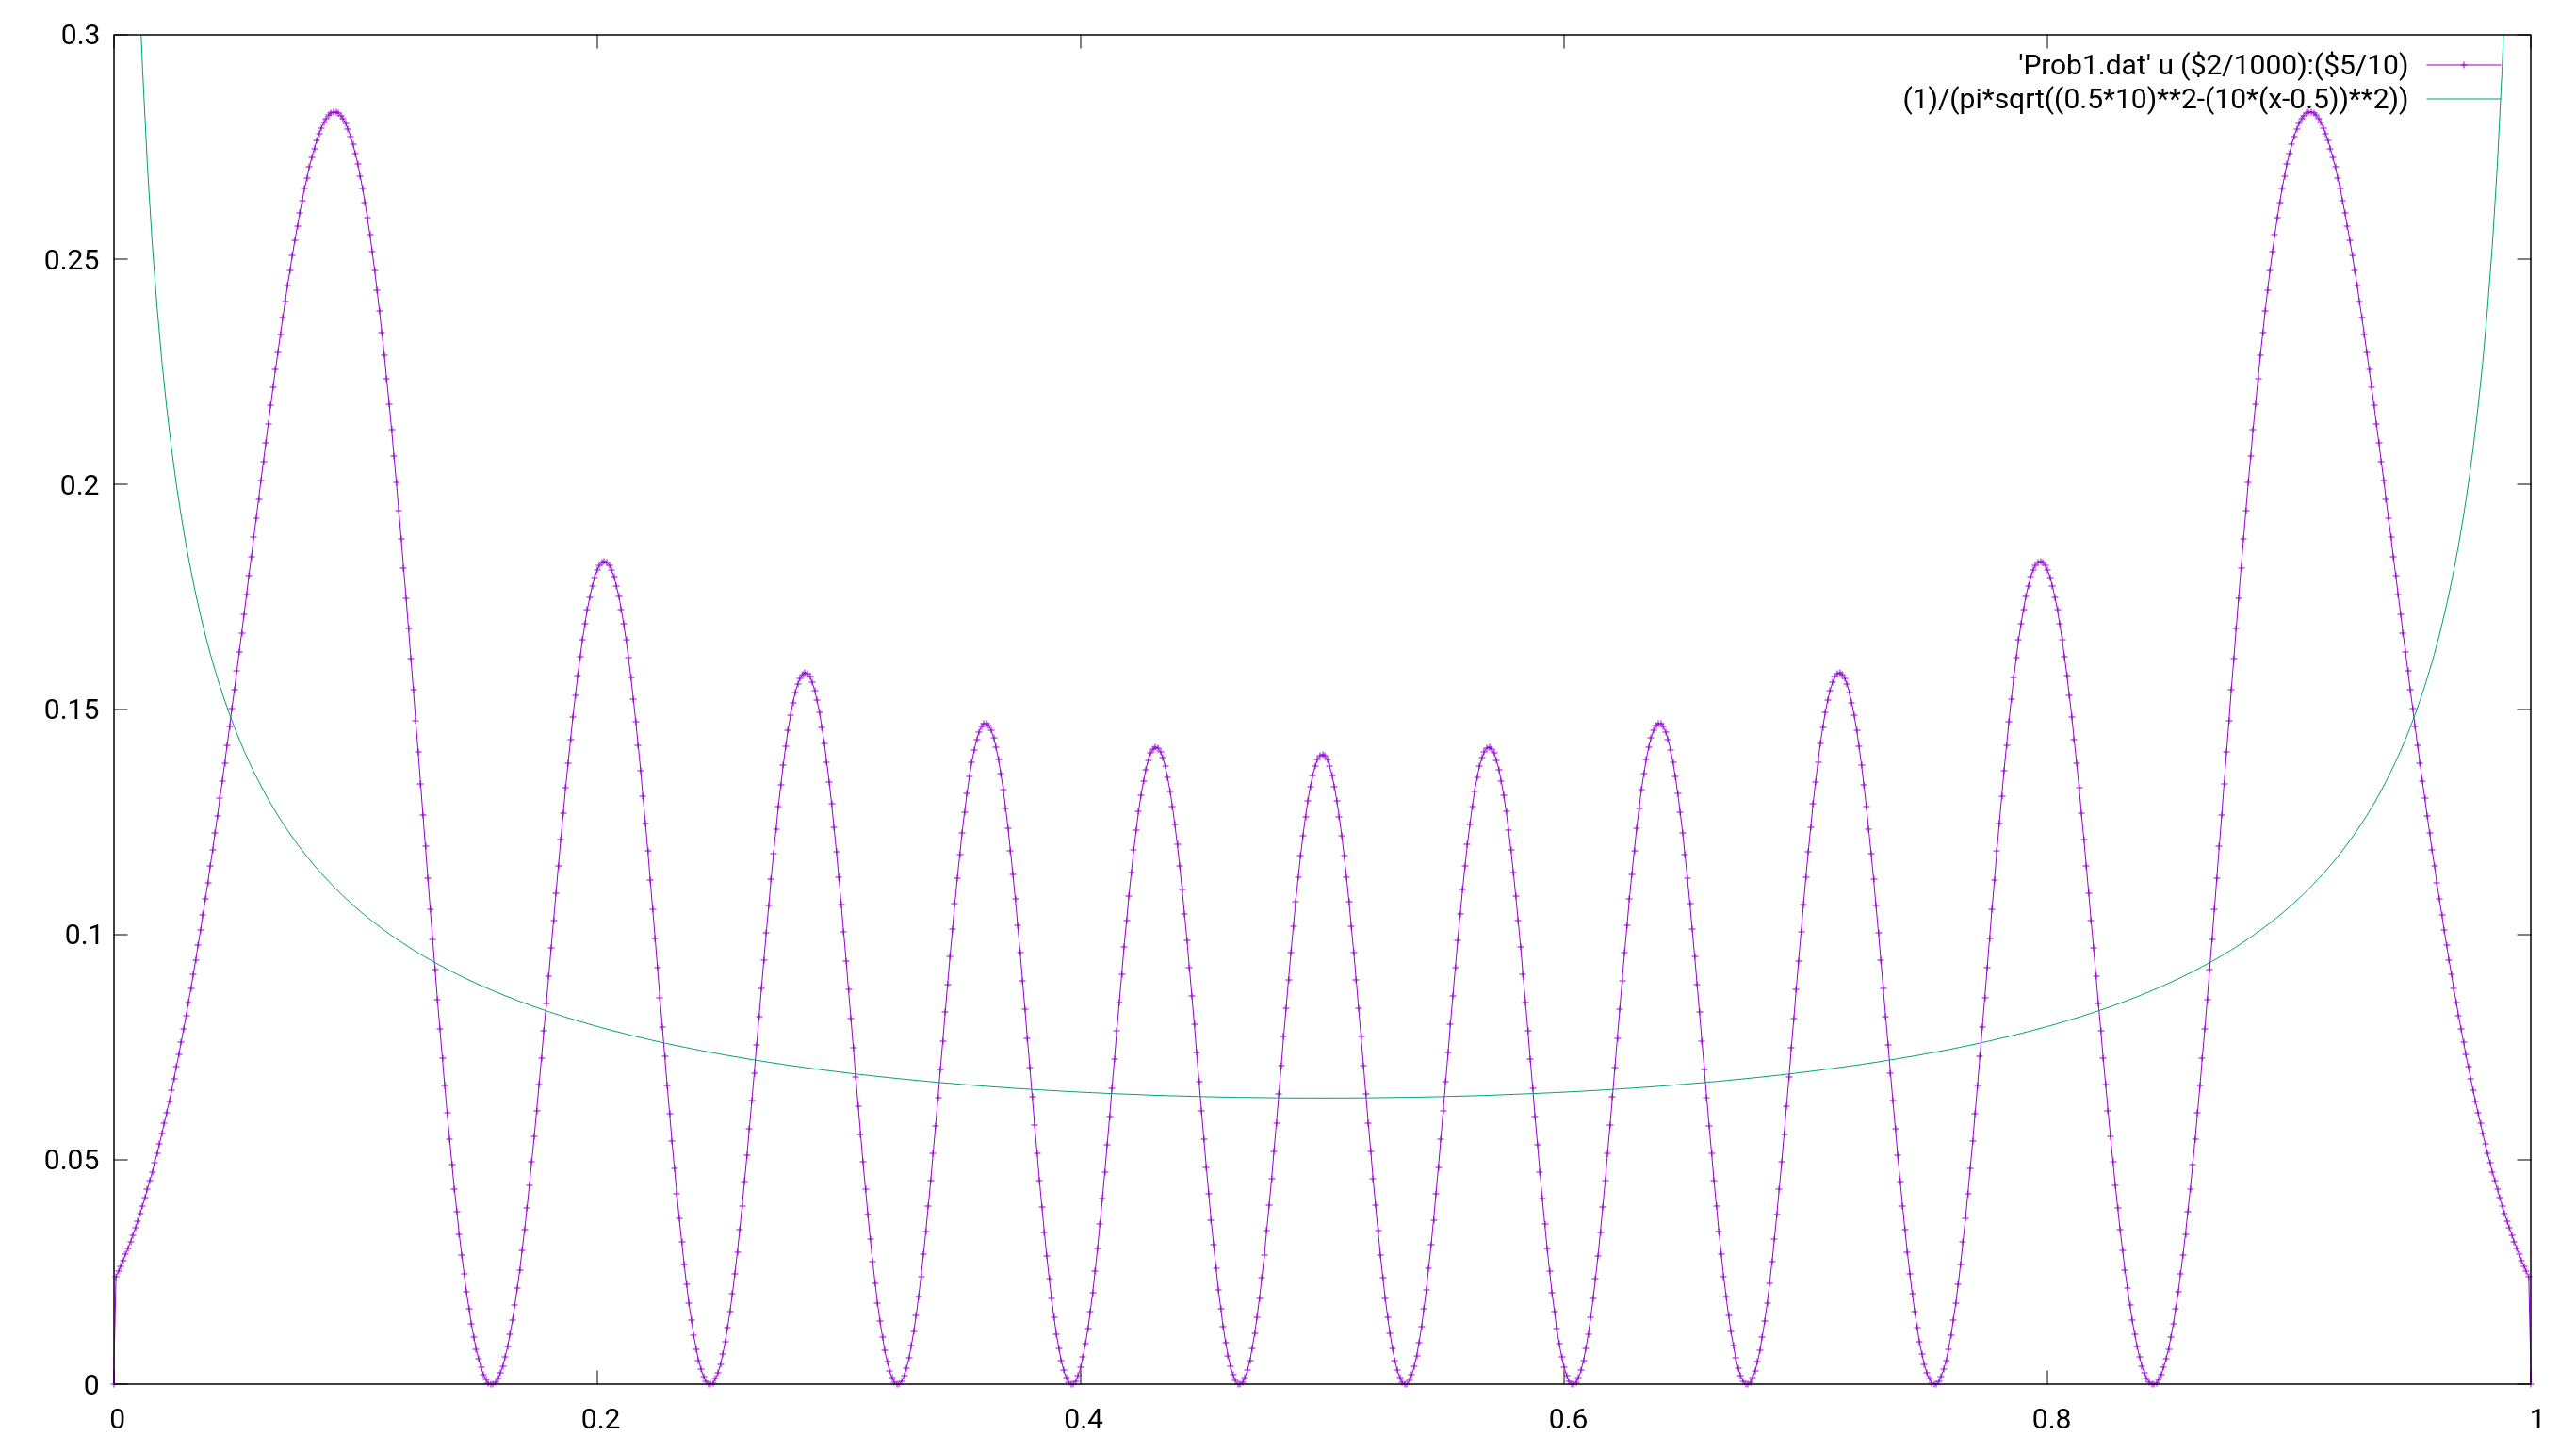
\includegraphics[width=0.775\textwidth]{Imagenes/ComPcyParmN10.png}}
    \subfigure[$P(x,t)$ para N=15 comparado con $P_C$.]{
        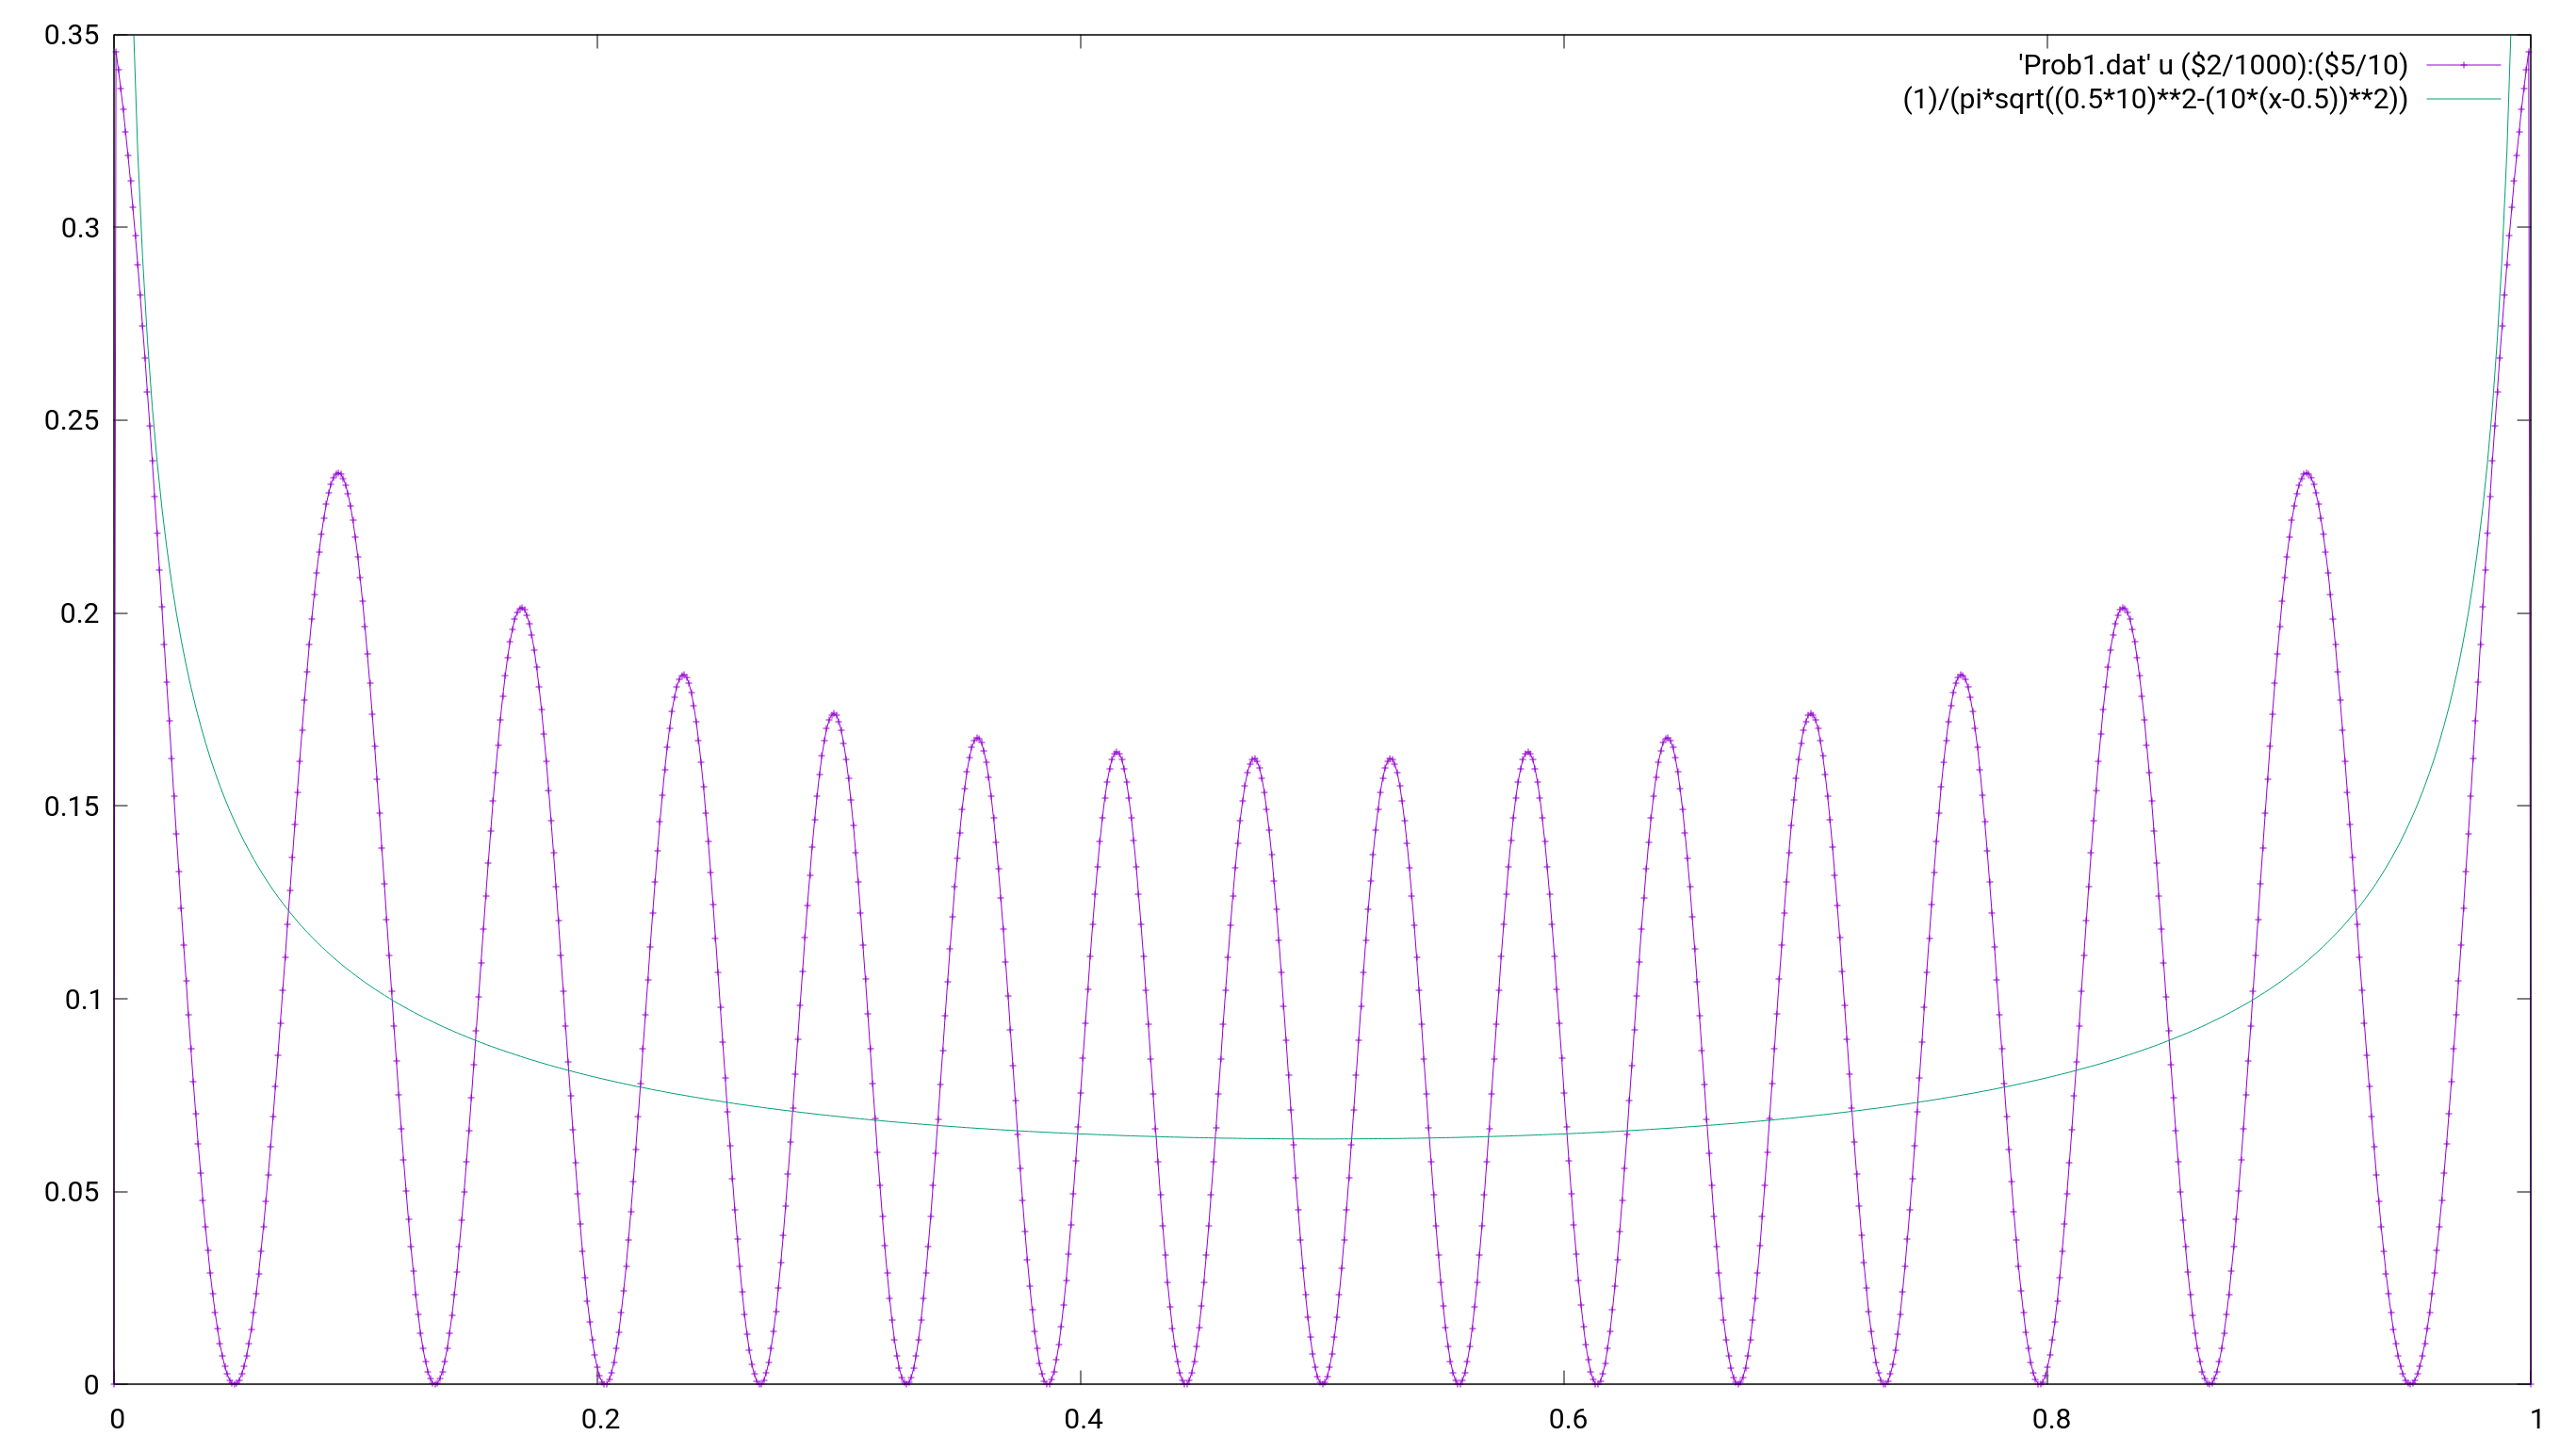
\includegraphics[width=0.775\textwidth]{Imagenes/ComPcyParmN15.png}}
    \subfigure[$P(x,t)$ para N=20 comparado con $P_C$.]{
        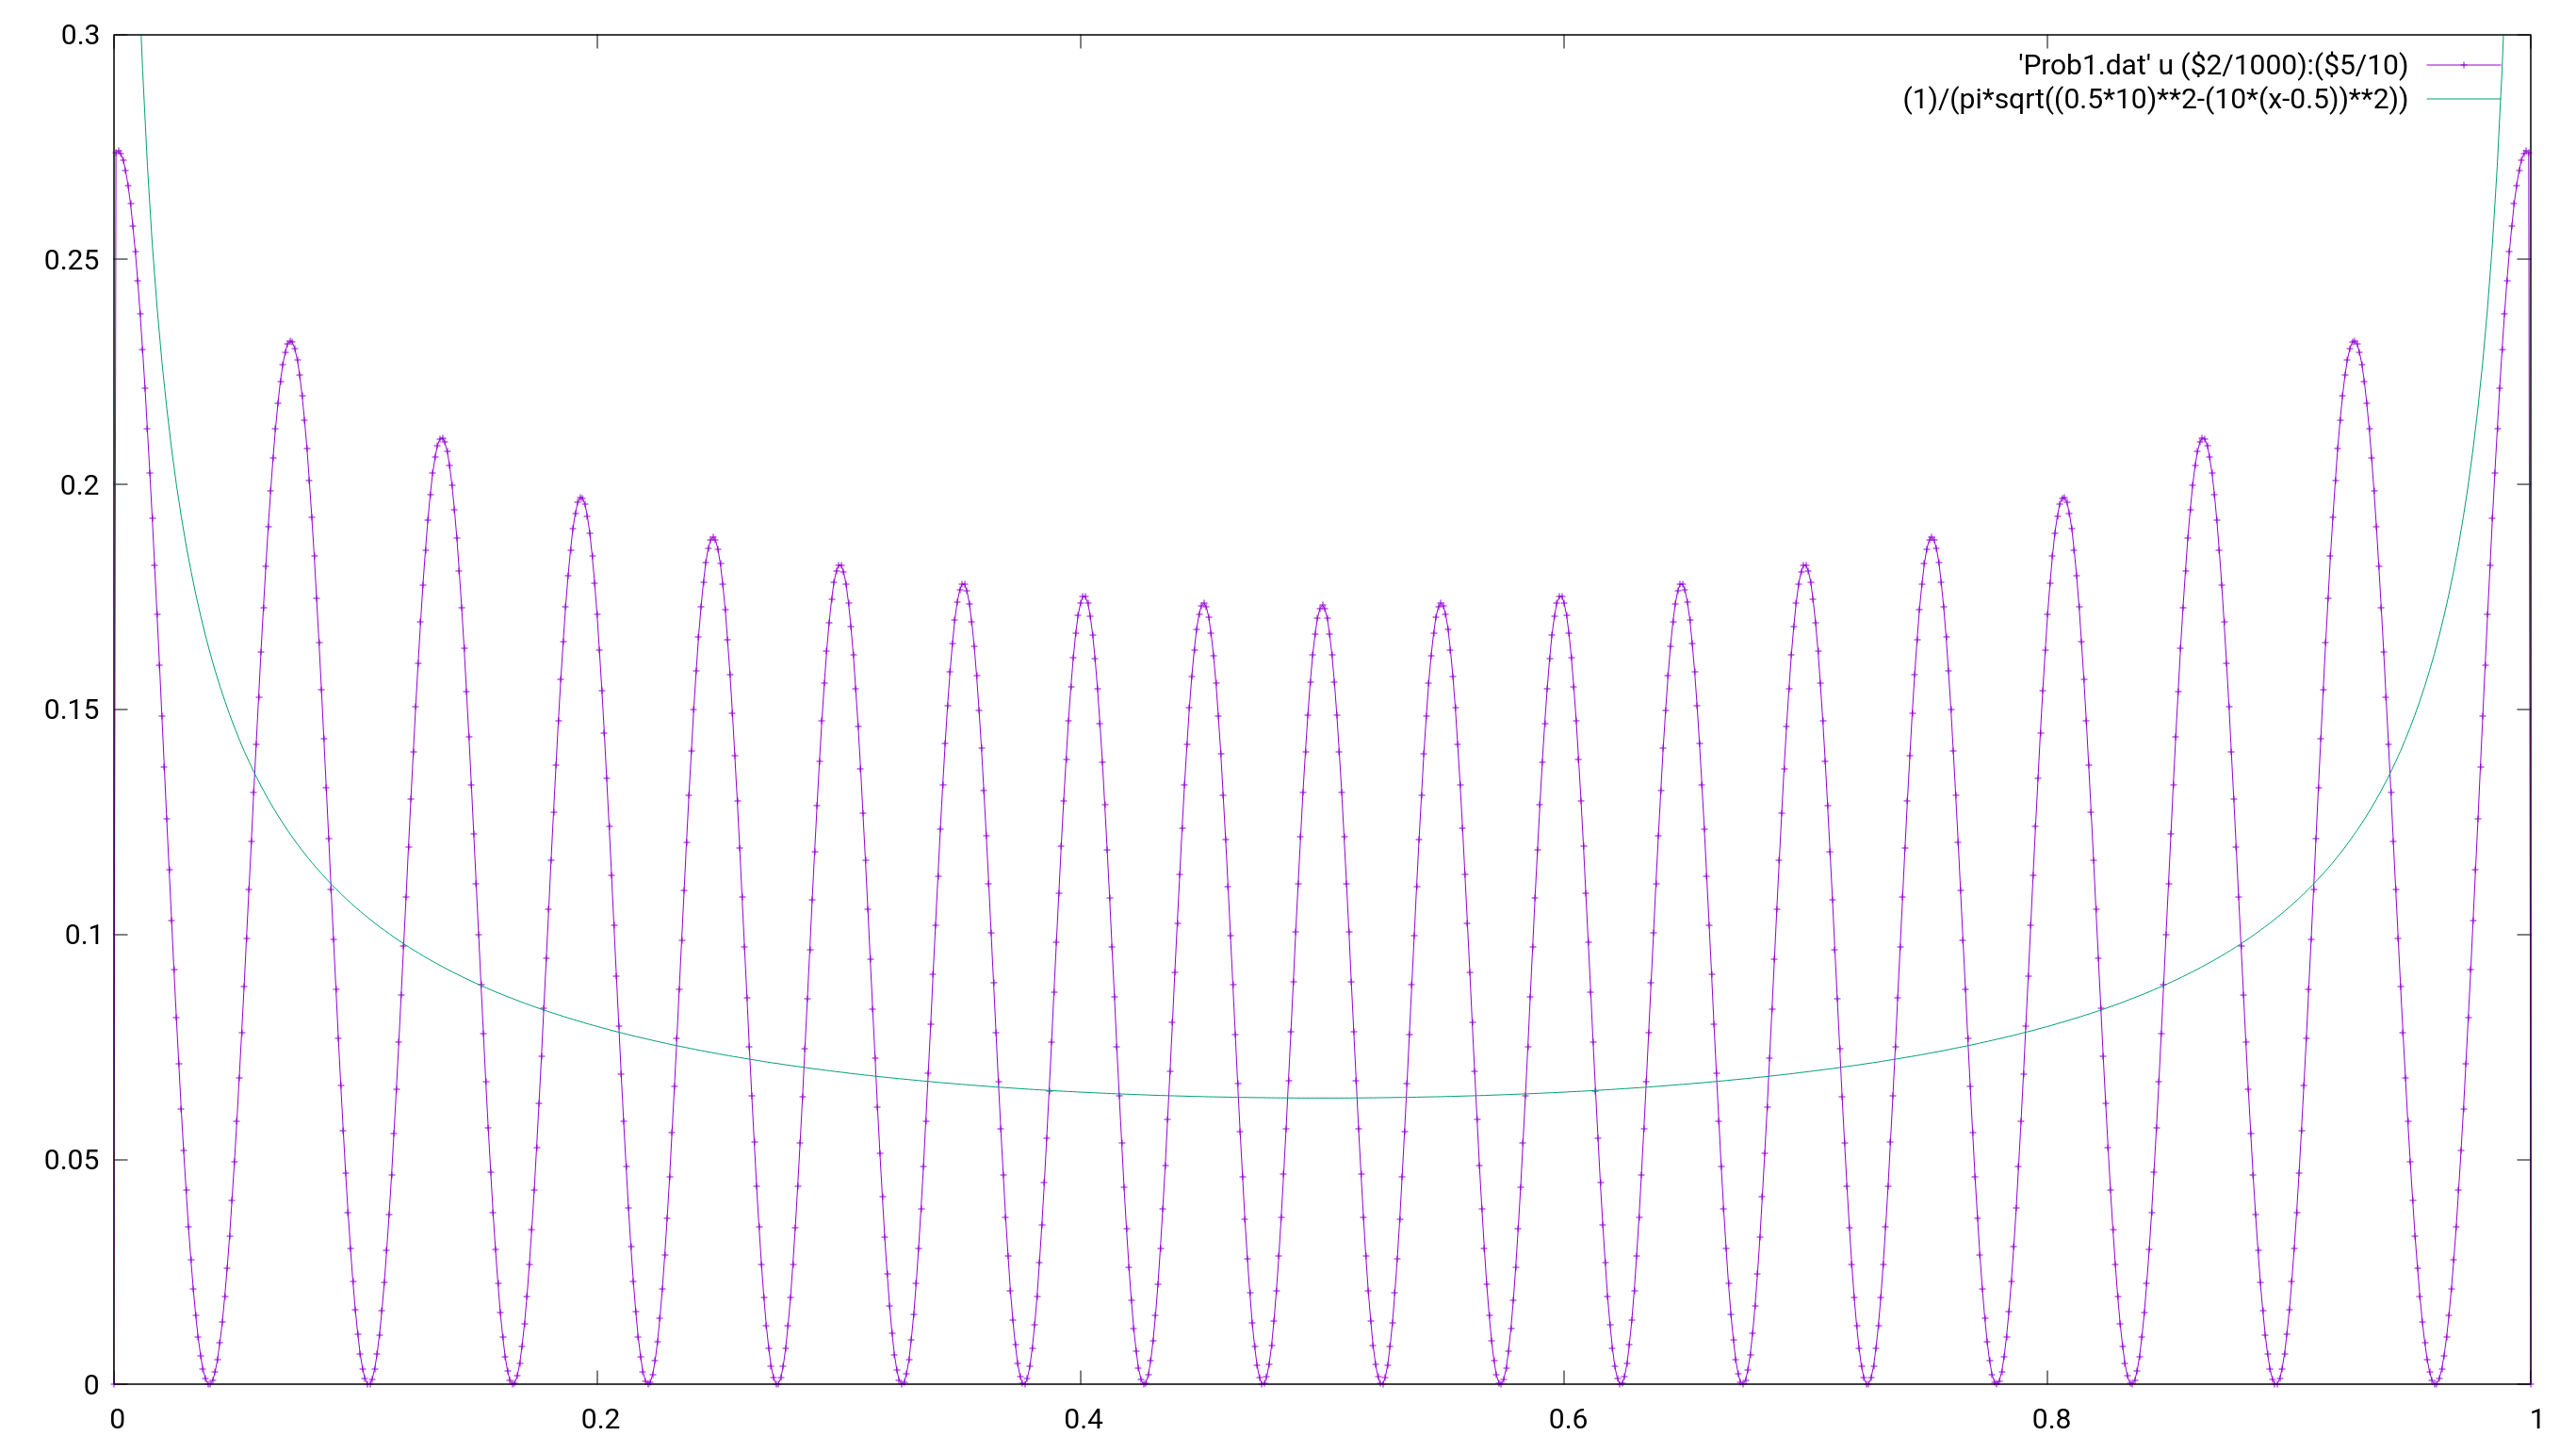
\includegraphics[width=0.775\textwidth]{Imagenes/ComPcyParmN20.png}}

  \end{center}
\end{figure}\\
Podemos denotar con bastante claridad cómo según nos vamos acercando a N=20, la densidad de probabilidades comienza a tomar forma de la probabilidad clásica. Quedando así demostrado el Principio de Correspondencia de Bohr.
\subsubsection{Comparación con es oscilador armónico clásica.}
Cuando tenemos un oscilador armónico en física clásica debemos tener en cuenta que pueden darse 3 casos: un oscilador ideal (el que vamos a suponer), sin perdidas de energía, un amortiguado, con sus propios casos, en los que se va perdiendo energía poco a poco y las oscilaciones se reducen poco a poco, y finalmente, el forzado, aquel al que se le aplica una fuerza para contrarrestar la energía que pierde o para aumenta el tamaño de las amplitudes.\\
Para que corresponda con el oscilador armónico cuántico, vamos a suponer que es una partícula en una caja que se mueve por la acción de un muelle, $k = mw^2$, es decir, en nuestro caso de $k=10000$, con velocidad angular $\omega = 200$, y $m=1/2$ y en una caja igual que el oscilador armónico cuántico de L=1. Por tanto sea la ecuación que describe el movimiento o la posición en el eje de la caja tal que:
\begin{equation*}
    F = m\frac{\delta^2x(t)}{\delta t^2} = - \nabla V(x) = -20000(x(t)-0.5) \hspace{2mm} y \hspace{2mm} x(t) = Acos(\omega t + \phi_0)
\end{equation*}
para adaptarlo tenemos que suponer que $A=0.5$, y debemos desplazar la función de onda al espacio entre 0 y L, tal que la partícula esté en el centro, es decir, sumamos un factor $x_0=0.5$. Para que comience a moverse en el centro tenemos que suponer que el desfase es $\pi/2$ para que $t=0$ es $x(0) = 0$ dando cómo resultado las siguientes ecuaciones tanto de la posición cómo de la velocidad:
\begin{equation*}
    x(t) = 0.5cos(200x) + 0.5 \hspace{2mm} y \hspace{2mm} v(t)=-100sen(200t)
\end{equation*}
Por tanto:
\begin{equation*}
    p = mv^2 = 5000sen^2(200t), \hspace{2mm} T = \frac{1}{2}p=2500sen^2(200t), \hspace{2mm}V = 10000(x-0.5)^2 \hspace{2mm} y \hspace{2mm} H = T+V
\end{equation*}
Se van a representar las gráficas correspondientes para todas las anteriores variables excepto para la velocidad en las siguientes gráficas para un lapso de tiempo t = 0.5. Finalmente se van a dar los valores medios tanto de la posición, cómo del momento y de la energía.\\
\begin{figure}[H]
    \centering
    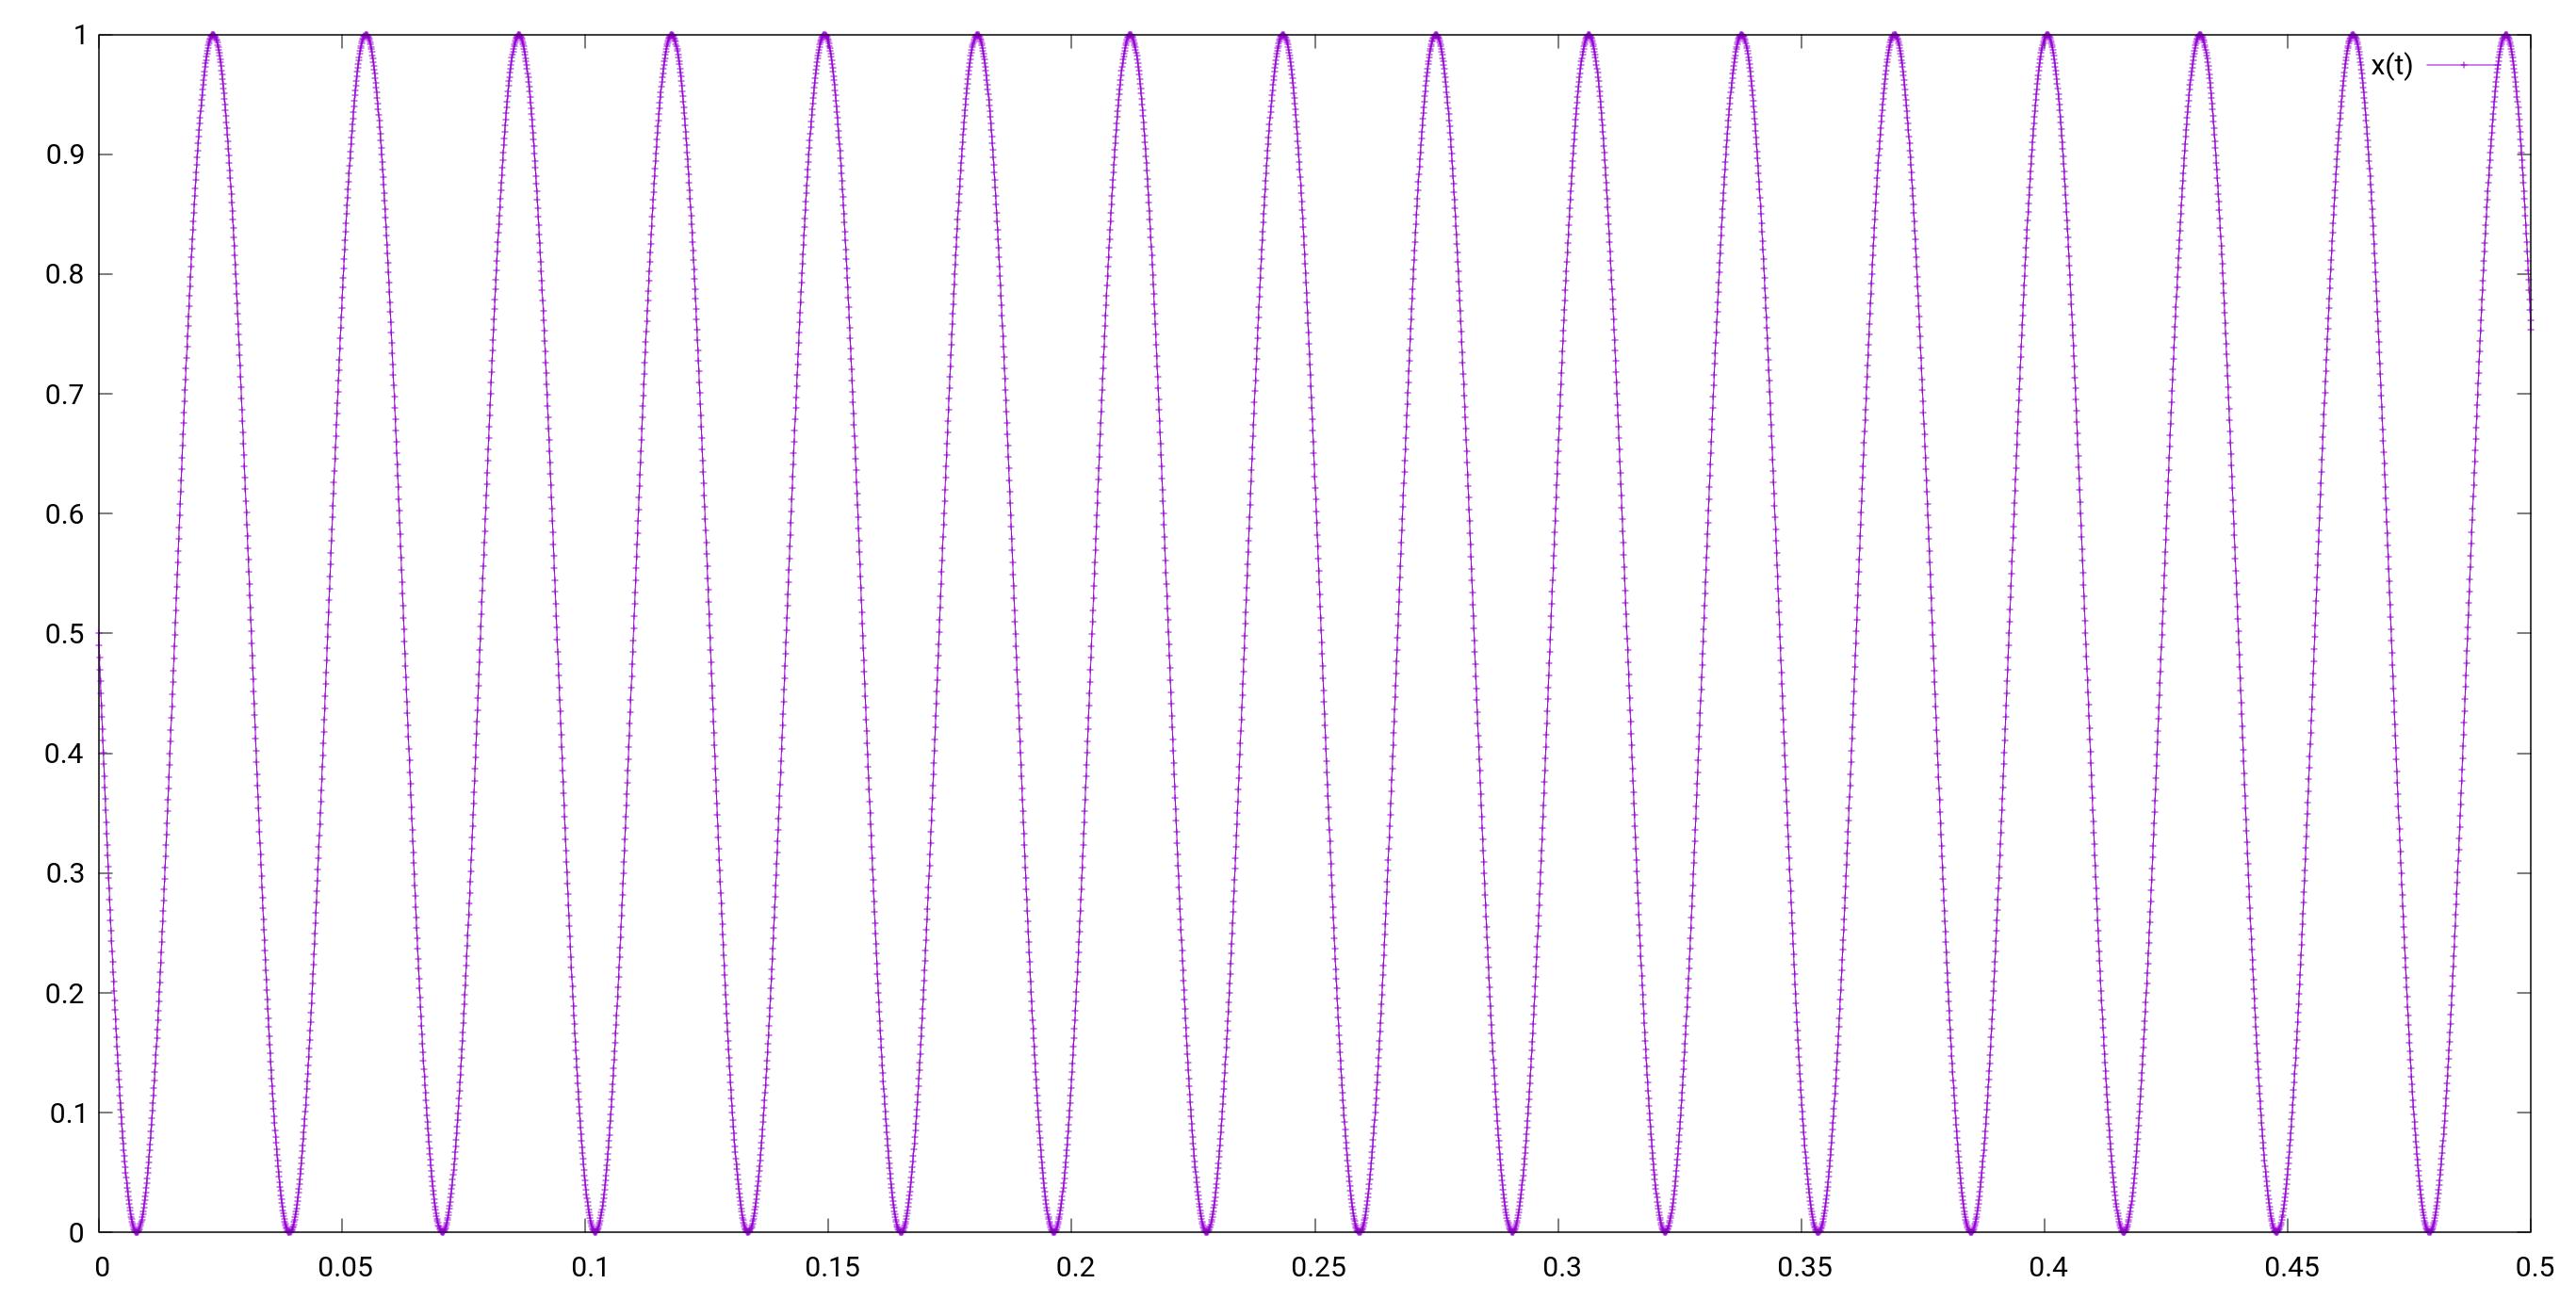
\includegraphics[width=0.775\textwidth]{Imagenes/XT.png}
    \caption{Imagen que representa variaciones de la posición de la partícula en el eje y cómo función del tiempo en el x de la gráfica.}
    \label{fig:enter-label}
\end{figure}
\begin{figure}
    \centering
    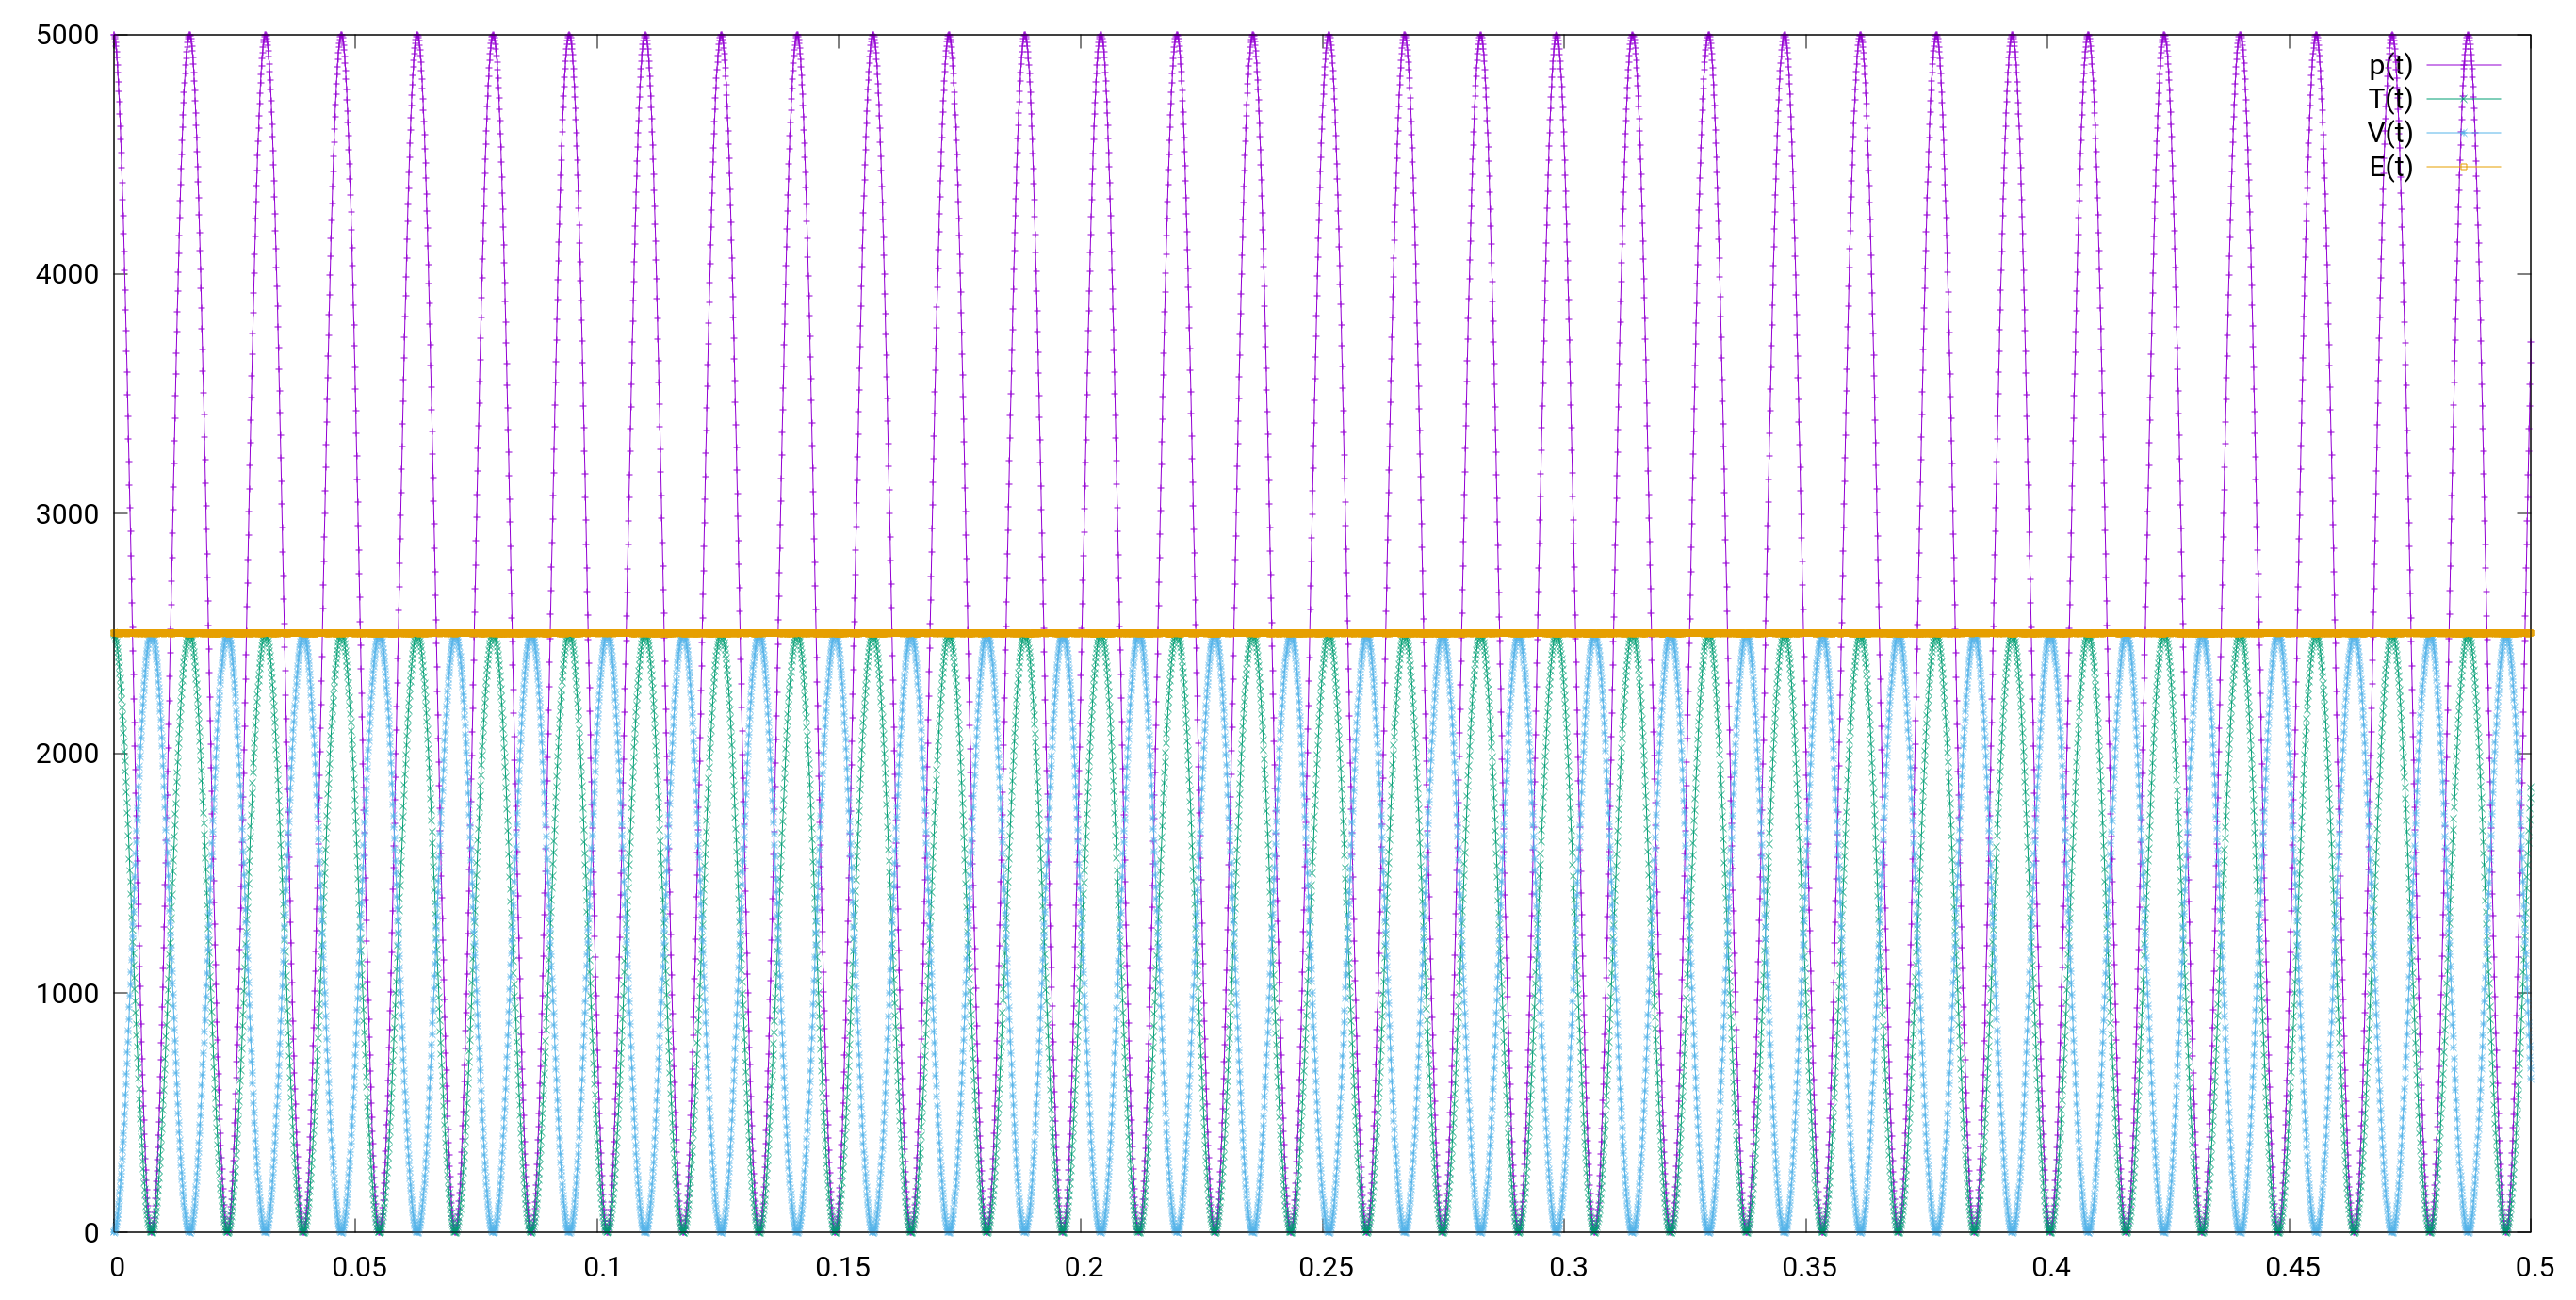
\includegraphics[width=1\textwidth]{Imagenes/ValoresOscArmClas.png}
    \caption{Imagen que representa variaciones del momento, y energías en el eje y cómo función del tiempo en el x de la gráfica.}
    \label{fig:enter-label}
\end{figure}\\
donde los valores medios son $<x> = 0.5$, $<p> \approx 2486.957$ y $<H> = 2500.5$.\\
Podemos ver que para el primer valor claramente es idéntico al oscilador armónico cuántico pero para el resto de valores existe una clara diferencia, pero tiene sentido que sean mucho mayores porque el sistema es mucho más grande. De hecho podemos comprobar cómo según aumentamos el número cuántico así lo hace tanto la energía cómo el momento. Por otro lado, podemos comprobar y entender cómo los valores medios de estás magnitudes varían a lo largo de los instantes de tiempo mientras que para entenderlo en el oscilador armónico cuántico es necesario obtener sus valores medios en cada instante de tiempo y posición. Si realizamos la media de dichos salen valores constantes en los tres casos para el oscilador clásico, cosa que obviamente no pasa para el momento medio en el caso del oscilador armónico cuántico, que va variando a lo largo del tiempo. Para el resto podemos ver que si corresponden. Aun así podemos concluir y visualizamos la clara diferencia que existe entre ambos modelos/casos.

\section{Conclusiones.}
El método numérico para aplicar la ecuación de Schrödinger a una función de onda, y posteriormente obtener gráficas y animaciones del desplazamiento de las mismas ondas es definitivamente de relevante importancia para entender y visualizar con mayor claridad este tipo de problemas, que a priori, no son tan intuitivos.\\

Partiendo de ecuaciones cómo la ecuación de Schrödinger, una función de onda cualquier dada y partiendo del Hamiltoniano, podemos obtener recursivamente y numéricamente el desarrollo de la función de onda para un tiempo y en un espacio dado. Podemos aplicarlo para diferentes tipos de onda pero en este caso se ha hecho hincapié en el oscilador armónico simple.\\
Se han tratado, estudiado y visualizado cómo evoluciona el sistema y las variaciones que tiene para las primeras 4 autofunciones del Hamiltoniano con un potencial dado (de números cuánticos 0, 1, 2 y 3), obteniendose cómo resultado lo que podemos ver las gráficas 1, 2, 3 y 4. Donde denotamos una ondas con distribución de probabilidades muy variables, con diferentes valores de la energía y del momento medio, pero todas conservan la posición media en el mismo valor, y la norma. También podemos denotar con bastante claridad cómo según aumentamos el número cuántico aumenta el número de vientres del sistema.\\
Por otro lado denotamos cómo calculando y obteniendo los valores teóricos y esperados para $\Delta x \Delta p$, primero comprobamos que se cumple el principio de Heisenberg, y que los valores teóricos que deberían obtenerse coinciden completamente con los obtenidos. Esto nos permite hacernos a la idea de lo preciso que este método y lo que cuadra con la teoría. Podemos denotarlo en la gráfica 5.\\

Por otro lado se ha estudiado cómo evoluciona el sistema si la función de onda inicial fuese una Gaussiana tipo, donde hemos denotado con bastante claridad que el potencial introduce un impulso en la onda que la hace moverse de una lado a otro si el potencial y la onda no están centrados en el mismo punto. También se ha visualizado cómo para una onda centrada en el potencial esta sufre variaciones en la amplitud de la misma, siendo esto principalmente denotable en la densidad de probabilidades. Y finalmente comprobamos que para un valor de la función igual al de la primera autofunción del Hamiltoniano obtenemos el mismo resultado. Gráficas 6, 7 y 8. Aun más reflejado lo podemos ver para $\Delta x \Delta p$ en la gráfica 9.\\

También se ha comprobado el Principio de Correspondencia de Bohr, es decir, que según vamos aumentando el número cuántico, más se asemeja la distribución de la densidad de probabilidades a la de la probabilidad clásica de encontrar una partícula en dicha posición. Mayor claridad en gráficas 10 y 11.\\

Finalmente se han comparado el oscilador armónico cuántico con un oscilador armónico clásico quedando con bastante claridad las diferencias que se producen salvo algunas similitudes. Las variaciones en el tiempo del oscilador armónico clásico da cómo resultado una posición media igual a la del cuántico, y un momento y energía medios de mayor magnitud, cosa que corresponde al aumento de los números cuánticos para el problema del oscilador armónico cuántico. Por el resto, las diferencias son notables.

\newpage
\begin{thebibliography}{}

\bibitem{}
schr-SLIDES$\_$ultimo.pdf. Física Computacional. Grado en Física. Prado.

\bibitem{}
problema$\_$osc$\_$arm$\_$cuant.pdf. Física Computacional. Grado en Física. Prado.

\bibitem{}
https://es.wikipedia.org/wiki/Ecuaci$\%$C3$\%$B3n\_$de\_$Schr$\%$C3$\%$B6dinger

\bibitem{}
https://es.wikipedia.org/wiki/Hamiltoniano$\_$(mec$\%$C3$\%$A1nica$\_$cu$\%$C3$\%$A1ntica)

\bibitem{}
https://es.wikipedia.org/wiki/Relaci$\%$C3$\%$B3n$\_$de$\_$indeterminaci$\%$C3$\_$$\%$B3n$\_$de$\_$Heisenberg

\bibitem{}
Capítulo 4 de Introduction to quantum mechanics de B.H. Bransden y C.J. Joachin.

\end{thebibliography}

\end{document}